%*****************************************
\chapter{Multi-scale techno-economic assessment of nitrogen recovery systems for swine operations}\label{ch:NitrogenTechs}
%*****************************************
\begin{refsection}[referencesCh6]
\section{Introduction}
The agricultural sector has experimented an industrialization process since the XIX century, pursuing the intensification of the agri-products and food production, i.e., increasing the agricultural production per unit of input resources, including land, labor and feed among others \citep{FAOethics2004}. During the last decades, the agricultural intensification is driven by a sustained increase in the population, the average income growth in both developed and developing countries, and the trade liberalization and logistics advancements leading the transnational trade of products \citep{baker2014trends}. As a result of this intensification process, the largest quantity and variety of agri-products in the human history is produced and distributed nowadays. However, multiple environmental challenges must be faced as a consequence of the industrialization of the agriculture and farming activities: soil depletion of nutrients and organic matter as consequence of mono-cropping, excessive and inefficient use of synthetic fertilizers to maintain high cropping yields, spatial concentration and inappropriate management of livestock manure, biodiversity loss, etc. 
Focusing in the context of nutrient management, the use of synthetic fertilizers, and the detachment of arable lands and livestock facilities decoupled the previous link where the organic waste from livestock activities were used as nutrient and organic matter supply for crops \citep{bouwman2009human}. This decoupling has created a dependency on mineral (phosphorus) and synthetic (nitrogen) fertilizers, and the adequate management of animal manure has become a serious problem for concentrated animal feeding operations (CAFOs). Therefore, there is disconnection between localized areas with large concentrations of organic waste containing nutrients, such as the intensive livestock facilities, and croplands demanding nitrogen and phosphorus
%to keep high yield rates which relies
relying in synthetic and mineral fertilizers to keep high yield rates. Due to the sparse location of the facilities and the high density of organic wastes, including manure and digestate, the transportation of these wastes for nutrients redistribution is challenging and expensive \citep{sampat2018technologies}. Therefore, the implementation of technologies and processes for the recovery of nutrients in a form suitable for easy transport and use in croplands is of utmost importance, restoring the circularity of agricultural nutrients usage disrupted by industrial practices. However, the selection of the most suitable technology for an individual facility is not a trivial process, but involves multiple dimensions, including the recovery efficiency, the effect of the scale on the economic performance of the process, and the environmental footprint of the different technologies. Some previous works assessing and comparing technologies have been performed, but they do not capture the effect of the economies of scale \citep{munasinghe2020nitrogen, de2019resource}, or they are limited to a few number of technologies \citep{bolzonella2018nutrients}.
%, or they are not focused in livestock waste \citep{beckinghausen2020removal}. 
\citet{beckinghausen2020removal} reports a lack of techno-economic analyses for nitrogen recovery techniques to identify the most suitable process according to the characteristics of each facility. In addition, the previous studies do not capture the effects of integrating these processes with anaerobic digestion systems for energy recovery.

%In this work, a systematic techno-economic analysis, including the scale effect on the economic performance is carried out for comparing the state-of-the-art technologies for nitrogen recovery from livestock waste, {\color{red}{i.e., transmembrane  chemisorption, ammonia evaporation and scrubbing, striping in packed tower, aeration stripping, MAPHEX, and struvite production.}} A material flow analysis (MFA) from waste collection to final treatment is combined with the are analyzed
In this work, six state-of-the-art technologies for nitrogen recovery from livestock waste, i.e., transmembrane  chemisorption, ammonia evaporation and scrubbing, striping in packed tower, MAPHEX, and struvite production, are systematically assessed and compared. Each system is evaluated performing a material flow analysis (MFA) of the whole process, from waste collection to the final treatment, and a techno-economic analysis (TEA) capturing the effect of the economies of scale on the cost of nitrogen recovery.
%through the development models for the calculation of the energy and mass balances, including the recovery yield; and for economic evaluation purposes. 
The objective is to determine the most adequate technologies to close the nutrients loop from livestock to crops, and the optimal conditions for the implementation of
%each one of
these systems. The processes for livestock waste treatment studied involve all stages from waste collection to the production of the nutrient-rich final product: manure preconditioning, optional biogas production valorization, solid-liquid separation of manure or digestate, and nutrients recovery. The assessment of such technologies is performed through detailed mathematical models of the processes based on first principles and experimental data, resulting in a flexible framework able to analyze different combinations and scales of technologies for the treatment of swine waste. The information obtained from the techno-economic assessment of nitrogen recovery technologies is key for the further development of policies to promote nutrient recovery and to mitigate the environmental footprint of swine farming activities.
%with special emphasis on the resiliency of the technology selected for each scenario, since there exist multiple variable factors that affect the performance of nutrient recovery facilities, e.g., the variability of waste composition, the prices of the products obtained, and the cost of the utilities required by each unit. Therefore, a flexible framework capable of assessing changes in input parameters is developed, allowing the study of the impact of the fluctuation of these variables on the results obtained, including the technical and economic performance of the different nutrient recovery technologies, and the selection of the optimal system. In addition, the application of potential government incentives is evaluated, determining the most cost-effective incentive policies to mitigate the economic impact of the nitrogen recovery facilities on the economies of the livestock facilities.  

\section{Methods}
\subsection{Livestock waste}
Swine manure generated by animals at different life stages have different composition, as well as a different waste generation ratio, i.e., waste mass generated per animal per day. Data reported by the US Department of Agriculture \citep{USDAWaste, Kellog2000} is used to determine the waste flow and composition as a function of the number of animals in a facility and their type, as listed in Table \ref{table:SwineWaste}. AU denotes animal units, which is defined as 1000 pounds (453.6 kg) of live animal \citep{animal_unit_definition}.

%\begin{table}[h] 
	%%	\begin{adjustwidth}{}{}
		%		\centering
		%		\caption{Swine waste characterization. Adapted from \protect\citet{USDAWaste, Kellog2000}.} \label{table:SwineWaste}
		%		\resizebox{\columnwidth}{!}{
			%		\begin{threeparttable}
				%		\begin{tabular}{@{}ccccccc@{}}
					%		\toprule
					%		Components        & Units     & Sow Gestating & Sow Lactating & Boar & Piglets Nursery & Piglets Grow\\to Finish \\ \midrule
					%		Animals:AU      & ratio     & 2.67          & 2.67          & 2.67 & 9.09            & 9.09                   \\
					%		Weight            & $\sfrac{\text{lb}}{\text{d AU}}$ & 25            & 59            & 19   & 88              & 65                     \\
					%		Volume            & $\sfrac{\text{ft\textsuperscript{3}}}{\text{d AU}}$ & 0.41          & 0.97          & 0.3  & 1.4             & 1.1                    \\
					%		Moisture          & \%wt  & 90            & 90            & 90   & 90              & 90                     \\
					%		TS                & $\sfrac{\text{lb}}{\text{d AU}}$ & 2.5           & 5.9           & 1.9  & 10              & 6.5                    \\
					%		VS                & $\sfrac{\text{lb}}{\text{d AU}}$ & 2.3           & 5.4           & 1.7  & 8.8             & 5.4                    \\
					%		N                 & $\sfrac{\text{lb}}{\text{d AU}}$ & 0.16          & 0.45          & 0.14 & 0.92            & 0.54                   \\
					%		P                 & $\sfrac{\text{lb}}{\text{d AU}}$ & 0.05          & 0.13          & 0.05 & 0.15            & 0.09                   \\
					%		K                 & $\sfrac{\text{lb}}{\text{d AU}}$ & 0.11          & 0.28          & 0.09 & 0.35            & 0.24                   \\
					%		N\textsubscript{inorganic}:N\textsubscript{total} & ratio     & 0.61          & 0.61          & 0.61 & 0.61            & 0.61                   \\
					%		N\textsubscript{organic}:N\textsubscript{total}   & ratio     & 0.39          & 0.39          & 0.39 & 0.39            & 0.39                   \\
					%		P\textsubscript{inorganic}:P\textsubscript{total} & ratio     & 0.58          & 0.58          & 0.58 & 0.58            & 0.58                   \\
					%		P\textsubscript{organic}:P\textsubscript{total}   & ratio     & 0.42          & 0.42          & 0.42 & 0.42            & 0.42                   \\ \bottomrule
					%	\end{tabular}
				%		\begin{tablenotes}
					%		\item AU: Animal units.
					%		\item TS: Total solids.
					%		\item VS: Volatile solids.
					%		\item N: Nitrogen.
					%		\item P: Phosphorus.
					%		\item K: Potassium.
					%	\end{tablenotes}
				%	\end{threeparttable}
			%	}
		%\end{table}
	
\begin{table}[h] 
%	\begin{adjustwidth}{}{}
	\centering
	\caption{Swine waste characterization. Adapted from \protect\citet{USDAWaste, Kellog2000}.} \label{table:SwineWaste}
	\resizebox{\columnwidth}{!}{
		\begin{threeparttable}
			\begin{tabular}{@{}ccccccc@{}}
				\toprule
				Components        & Units     & Sow Gestating & Sow Lactating & Boar & Piglets Nursery & Piglets Grow\\to Finish \\ \midrule
				Animals:AU      & ratio     & 2.67          & 2.67          & 2.67 & 9.09            & 9.09                   \\
				Weight            & $\sfrac{\text{kg}}{\text{d AU}}$ & 11.34            & 26.76            & 8.62   & 39.92              & 29.48                     \\
				Volume            & $\sfrac{\text{m\textsuperscript{3}}}{\text{d AU}}$ & 0.012          & 0.027          & 0.0085  & 0.040            & 0.031                    \\
				Moisture          & \%wt  & 90            & 90            & 90   & 90              & 90                     \\
				TS                & $\sfrac{\text{kg}}{\text{d AU}}$ & 1.13           & 2.68           & 0.86  & 4.54              & 2.95                    \\
				VS                & $\sfrac{\text{kg}}{\text{d AU}}$ & 1.04           & 2.45           & 0.77  & 3.99             & 2.45                    \\
				N                 & $\sfrac{\text{kg}}{\text{d AU}}$ & 0.073          & 0.20          & 0.064 & 0.42            & 0.24                   \\
				P                 & $\sfrac{\text{kg}}{\text{d AU}}$ & 0.023          & 0.059          & 0.023 & 0.068            & 0.041                   \\
				K                 & $\sfrac{\text{kg}}{\text{d AU}}$ & 0.050          & 0.13          & 0.041 & 0.16            & 0.11                   \\
				N\textsubscript{inorganic}:N\textsubscript{total} & ratio     & 0.61          & 0.61          & 0.61 & 0.61            & 0.61                   \\
				N\textsubscript{organic}:N\textsubscript{total}   & ratio     & 0.39          & 0.39          & 0.39 & 0.39            & 0.39                   \\
				P\textsubscript{inorganic}:P\textsubscript{total} & ratio     & 0.58          & 0.58          & 0.58 & 0.58            & 0.58                   \\
				P\textsubscript{organic}:P\textsubscript{total}   & ratio     & 0.42          & 0.42          & 0.42 & 0.42            & 0.42                   \\ \bottomrule
			\end{tabular}
			\begin{tablenotes}
				\item AU: Animal units.
				\item TS: Total solids.
				\item VS: Volatile solids.
				\item N: Nitrogen.
				\item P: Phosphorus.
				\item K: Potassium.
			\end{tablenotes}
		\end{threeparttable}
	}
\end{table}

\subsection{Nitrogen management systems assessment framework} \label{section:NitrogenManagModels}
Swine manure processing involves several stages from manure collection to resources recovery, as shown in Figure \ref{fig:techs_diagrams}. In this section the modeling details of each stage are drawn.
\begin{figure}[h]
	\centering
	%	\begin{subfigure}[t]{0.5\linewidth}
		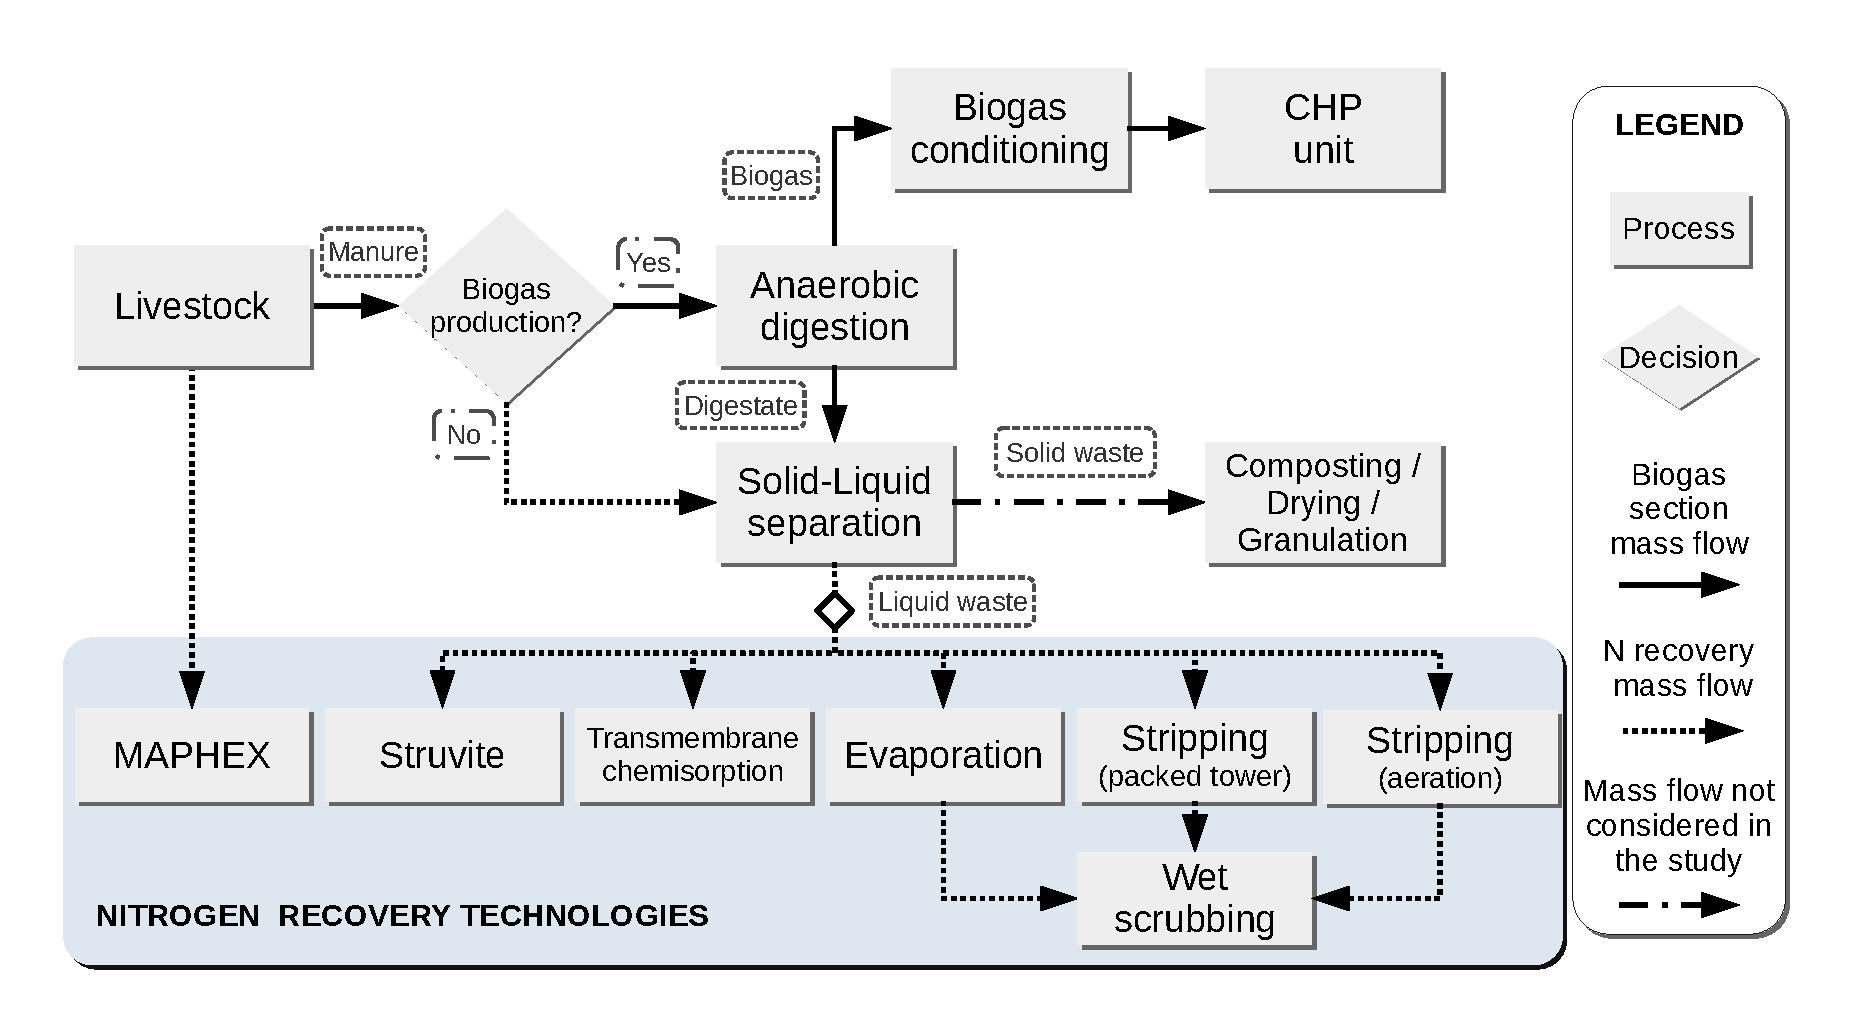
\includegraphics[width=0.75\linewidth, trim={1cm 1cm 1cm 1cm},clip]{gfx/Chapter6/Process_Flowsheet2.pdf} 
		\caption{Flowchart of the processes assessed for the processing of livestock waste}
		\label{fig:techs_diagrams}
	\end{figure}

\subsubsection{Anaerobic digestion}
Swine manure can be processed in an anaerobic digestion (AD) unit for the production of biogas and digestate. These materials can be further processed to recover valuable resources, such as electricity and thermal energy from biogas, and nutrients from digestate. As a result of the digestion process, the organic and inorganic fractions of nutrients (i.e., nitrogen and phosphorus) vary due to the partial mineralization of the organic fraction of nitrogen and phosphorus. Therefore, the amount of inorganic nutrients in the digestate is larger than in raw manure, as shown in Table \ref{table:ADWaste} \citep{fangueiro2020available}. In addition, the amount of total solids decreases as a consequence of the transformation of volatile solids into biogas. AD process is typically carried out either at mesophilic (25 and 45 \textdegree C) and thermophilic (45 and 50 \textdegree C) temperatures and atmospheric pressure, with retention times between 30-40 and 15-20 days respectively. There also exist low temperature digestion at psychrophilic conditions ($<$ 25 \textdegree C), although it involves longer retention times between 70 and 80 days. The higher the temperature, the shorter the retention time \citep{Seadi2008}. A digestion temperature  of 40 \textdegree C and a retention time $\left( {HRT}_{\text{AD}} \right) $ of 21 days have been assumed in this work \citep{bolzonella2018nutrients}. 
%In Table ?? the variations in the organic and inorganic fractions of nutrients are 

\begin{table}[h] 
	\centering
	\caption{Variation of the inorganic fraction of nutrients biogas generation after anaerobic digestion of swine waste. Adapted from \protect\citet{fangueiro2020available}.} \label{table:ADWaste}
	\begin{threeparttable}
		\begin{tabular}{@{}cc@{}}
			\toprule
			Parameter      & Variation (\%) \\ \midrule
			TS             & -45            \\
			VS             & -52.5          \\
			N\textsubscript{inorganic}         & 45             \\
			P\textsubscript{inorganic}         & 16             \\
			%		$\sfrac{\text{m}^3_{\text{biogas}}}{\text{kg}_{\text{VS}}}$ & 0.57           \\
			\bottomrule
		\end{tabular}
		\begin{tablenotes}
			\item TS: Total solids.
			\item VS: Volatile solids.
			\item N: Nitrogen.
			\item P: Phosphorus
			.
		\end{tablenotes}
	\end{threeparttable}
\end{table}

The composition of biogas produced is based on data reported by \citet{Ciborowski}. The energy requirements of the AD unit $\left( Q_{\text{digester}} \right)$, described in Eq  \ref{eq:general1Manuscript}, comprise the energy required for substrate warming up from ambient temperature (assumed to be 12 \textdegree C) $\left( Q_{\text{waste}} \right)$ to the digestion temperature (40 \textdegree C),
%Eq. , 
and the energy supplied to offset the digester heat losses $\left( Q_{\text{losses}} \right)$.
%, {\color{blue}{Eq. \ref{eq:Qwaste} and \ref{eq:Qlooses} of the Supplementary Material}} respectively. The global heat transfer coefficients ($U$) for the different digester surfaces are collected in Table \ref{table:AD_U}. The area of different surfaces is estimated through preliminar equipment design, Eqs. \ref{eq:Vdigester1} to \ref{eq:Aroof}, assuming a maximum digester of 6000 m\textsuperscript{3} \citep{6000AD}. The installation of multiple digestion units is considered if the waste flow exceed this capacity.
{\color{blue}{The details of the energy balance to the AD unit can be found in the Supplementary Material, Eqs. \ref{eq:general1} to \ref{eq:Aroof}.}} A maximum digester size $\left( n_{\text{AD, }max} \right)$ of 6000 m\textsuperscript{3} is assumed \citep{ADSize}.

\begin{align}
	& Q_{\text{digester}} = Q_{\text{waste}} + Q_{\text{losses}} \label{eq:general1Manuscript}
	%	\\
	%	& Q_{\text{waste}} = \dot{m}_{\text{waste}} \cdot c_{p} \cdot \left(T_{\text{digestion}} - T_{\text{ambient}}\right) \label{eq:Qwaste} \\
	%	& Q_{\text{losses}} = \sum_{i} U_{i} A_{i} \left(T_{\text{digestion}} - T_{\text{ambient}}\right)\label{eq:Qlooses}, \forall i  \in \{\text{roof, walls, floor}\}
\end{align}

%\begin{table}[h] 
	%	\centering
	%	\caption{Anaerobic digester design parameters. \protect\citep{ADPennState}.} \label{table:AD_U}
	%	%	\begin{threeparttable}
		%	\begin{tabular}{@{}ccc@{}}
			%		\toprule
			%		\multicolumn{1}{c}{Parameter} & Unit  & \multicolumn{1}{c}{Value} \\ \midrule
			%		$U_{\text{floor}}$                        & $\sfrac{\text{W}}{\text{m}^2 \text{ K}}$     & 2.85                      \\
			%		$U_{\text{wall}}$                         & $\sfrac{\text{W}}{\text{m}^2 \text{ K}}$     & 0.39                      \\
			%		$U_{\text{roof}}$                         & $\sfrac{\text{W}}{\text{m}^2 \text{ K}}$     & 0.3                       \\
			%		$V_{\text{max}}$                         & m$^3$    & 6000                      \\
			%		$V_{\text{freeboard}}$                   & \%    & 30                        \\
			%		$HRT$                           & days  & 21                        \\
			%		$D_{\text{digester}}$:$H_{\text{digester}}$                           & ratio & 1.1                       \\
			%		$A_{\text{roof}}$:$A_{\text{floor}}$                  & ratio & 1.62                      \\ \bottomrule
			%	\end{tabular} 
		%	%		\begin{tablenotes}
			%	%			\item TS: Total solids.
			%	%			\item VS: Volatile solids.
			%	%		\end{tablenotes}
		%	%	\end{threeparttable}
	%\end{table}
%
%\begin{align}
	%	& V_{\text{digester}} = \frac{\dot{m}_{\text{waste}}}{\rho_{\text{waste}}} \cdot HRT \cdot \left(1 + \frac{V_{\text{freeboard}}}{100}\right) \label{eq:Vdigester1}\\
	%	& V_{\text{digester}} = A_{\text{floor}} \cdot \frac{D_{\text{digester}}}{D_{\text{digester}}:H_{\text{digester}}} \label{eq:Vdigester2} \\
	%	& A_{\text{floor}} = \pi \cdot \frac{D_{\text{digester}}^2}{4} \label{eq:Afloor} \\
	%	& A_{\text{wall}} = 2 \pi \cdot \frac{D_{\text{digester}}}{2} \cdot \frac{D_{\text{digester}}}{D_{\text{digester}}:H_{\text{digester}}} \label{eq:Awall}\\
	%	& A_{\text{roof}} = A_{\text{floor}} \cdot \left(A_{\text{roof}}:A_{\text{floor}}\right) \label{eq:Aroof}
	%\end{align}

%As shown in Figure \ref{fig:AD_size_2cost}, 
Correlations for capital expenditures (CAPEX) and operating expenses (OPEX) estimation as a function of animal units have been developed based on data reported by the USDA \citep{USDAOM}, as shown in Eqs. \ref{eq:nAD}-\ref{eq:OM_costs} and Figure \ref{fig:AD_size_2cost} of the Supplementary Material, where $\dot{m}_{digestate}$ denotes the digestate flow and $AU$ the number of animal units. It should be noted that operating and management (O\&M) cost does not include the capital cost amortization.
%\begin{figure}[H]
%	\centering
%	%	\begin{subfigure}[t]{0.5\linewidth}
	%	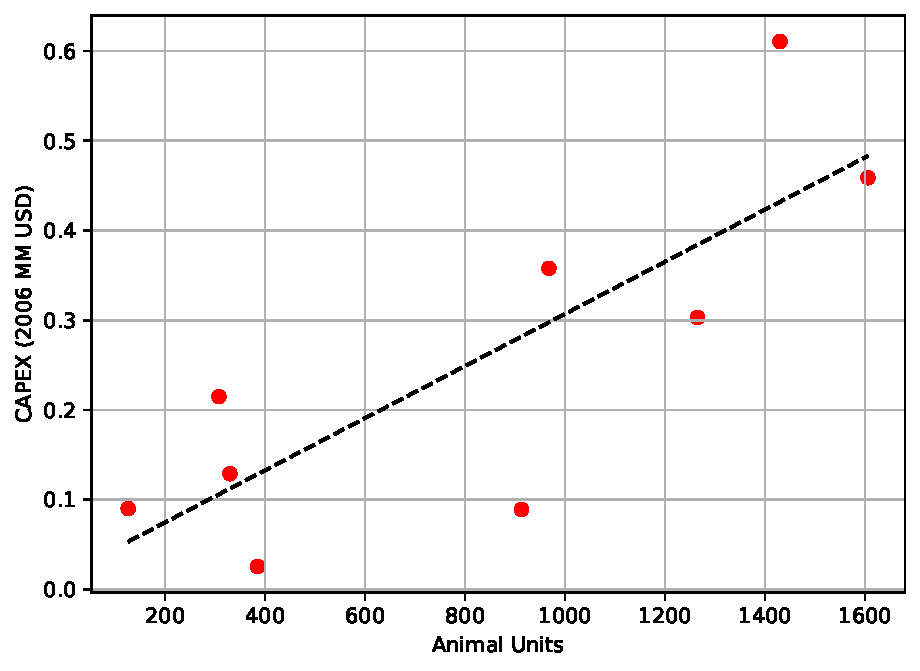
\includegraphics[width=0.6\linewidth, trim={0cm 0cm 0cm 0cm},clip]{AD_SizeCost_Swine.pdf} 
	%	\caption{Flowchart of the processes assessed for the processing of livestock waste}
	%	\label{fig:AD_SizeCost_Swine}
	%\end{figure}

%\begin{figure}[H]
	%	\centering
	%	\begin{subfigure}[t]{0.48\textwidth}
		%		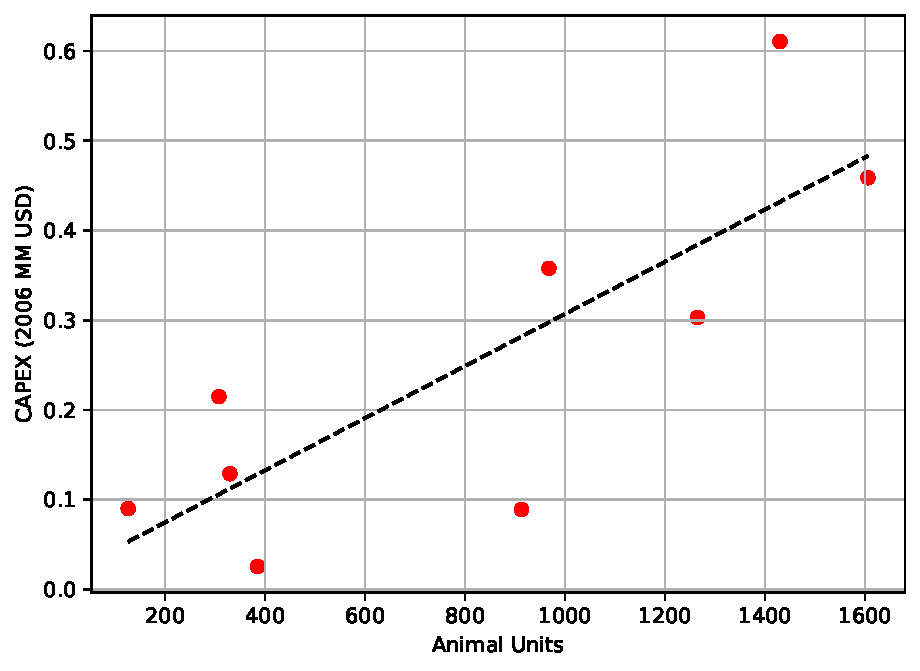
\includegraphics[width=\textwidth, trim={0cm 0cm 0cm 0cm},clip]{AD_SizeCost_Swine.pdf}
		%		\caption{Cost of AD units as a function of animal units.}
		%		\label{fig:AD_SizeCost_Swine}
		%	\end{subfigure}
	%	\quad
	%	\begin{subfigure}[t]{0.47\textwidth}
		%		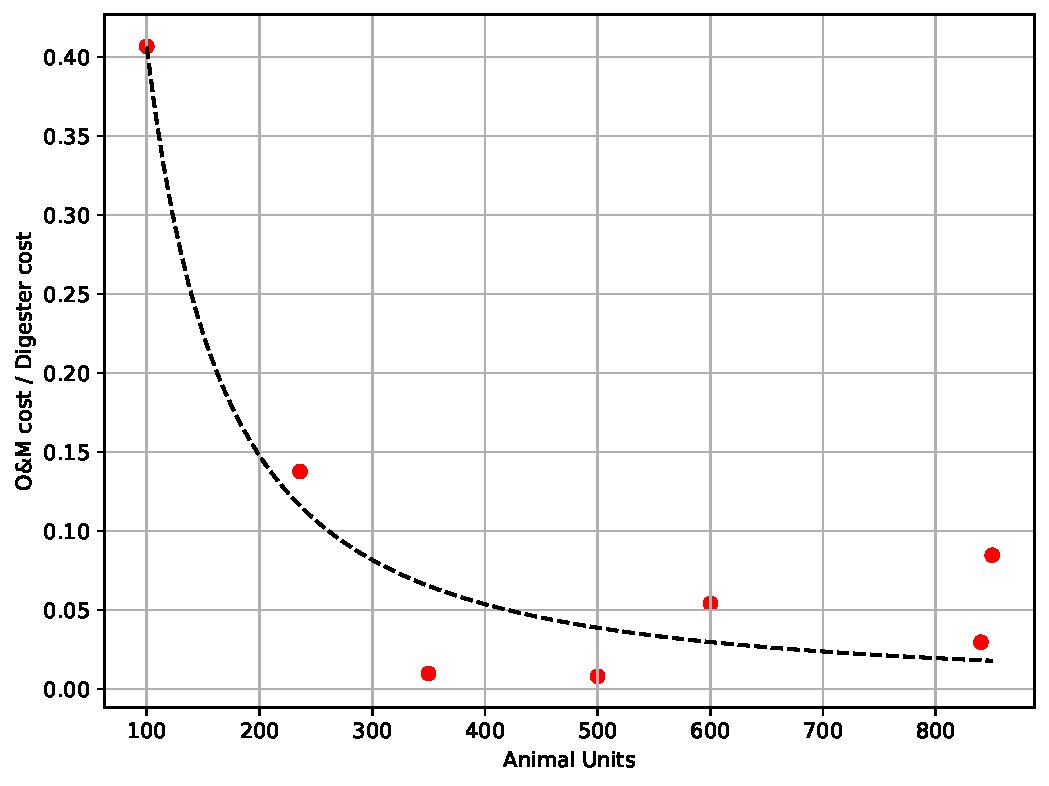
\includegraphics[width=\textwidth]{AD_size_OM_Unit_cost.pdf} 
		%		\caption{O\&M costs as a function of animal units.}
		%		\label{fig:AD_size_OM_Unit_cost}
		%	\end{subfigure}
	%	
	%	\caption{Correlations between AD capital and O\&M costs, and the number of cattle in the livestock facility. Data from \protect\citet{USDA_OM}.}
	%	\label{fig:AD_size_2cost}
	%\end{figure}

\begin{align} 
	& n_{\text{AD}} = \ceil*{\frac{\dot{m}_{digestate} \cdot HRT_{\text{AD}}}{n_{\text{AD, }max}}} \label{eq:nAD} \\
	& \text{CAPEX (MM USD (2019))} = \left(2.9069 \cdot 10^{-4} \cdot AU+0.01625\right) \cdot 1.216 \label{eq:inv_costs}\\ \nonumber\\
	%	& \frac{\text{O\&M}} {\text{Installation cost}} \text{ ratio} = \frac{15858.710}{(1+\left(N_{animals} \cdot 13.917\right)^{1.461}} \label{eq:OM_costs}\\ \nonumber\\
	& \text{OPEX } \left(\frac{\text{MM USD (2019)}}{\text{year}}\right) = \left(\frac{15.858\cdot 10^{3}}{1+\left(AU \cdot 13.917\right)^{1.461}}\right) \cdot \text{CAPEX} \label{eq:OM_costs}
	%	& \frac{\text{O\&M}} {\text{CAPEX}} \text{ ratio} = \frac{15.858\cdot 10^{3}}{(1+\left(AU \cdot 13.917\right)^{1.461}} \label{eq:OM_costs}\\ \nonumber\\
	%	& \text{OPEX } = \text{O\&M costs} + \frac{\text{Investment cost}}{\text{Plant lifetime}} \label{eq:OM_inv_costs}
\end{align}

\subsubsection{Biogas conditioning}
The raw biogas generated is conditioned to remove
%the main harmful elements within it. 
its impurities. Most of moisture is removed through condensation by compressing and cooling down the biogas stream. H\textsubscript{2}S is removed by using a fixed bed of Fe\textsubscript{2}O\textsubscript{3}, capturing the hydrogen sulfur
%in the form of 
as Fe\textsubscript{2}S\textsubscript{3}. The bed can be regenerated using the oxygen contained in air, leading to the formation of elementary sulfur \citep{ryckebosch2011techniques}. Ammonia and remaining moisture are removed through a pressure swing adsorption (PSA) system. For both processes, two adsorption units are typically installed in-parallel arrangement, so that one unit is in operation while the other bed is undergoing regeneration. Removal yields of 100\% have been assumed. More details can be found in {\color{blue}{Section \ref{section:BiogasConditioningNRecovery} of the Supplementary Material.}}

\subsubsection{Combined heat and power generation}
Biogas is valorized using a combined heat and power (CHP) unit to produce electricity and heat, which can be used to cover the thermal energy demand of the AD unit, and also for the nitrogen recovery processes if a source of heat is needed, e.g., ammonia evaporation. The energy recovered from biogas is estimated through its low heating value (LHV). LHV of biogas is a function of methane content, and it can be estimated using Eq. \ref{eq:LHV} \citep{BiogasLHV}, where $x_{\text{CH4}}$ refers to the methane mass fraction. Biogas combustion in the CHP unit is performed considering a 20\% air excess.

\begin{align}
	& LHV_{\text{biogas}} \left(\sfrac{\text{J}}{\text{m}^3}\right)= -46.26 \cdot 10^6 \cdot x_{\text{CH4}}^2 + 70.87 \cdot 10^6 \cdot x_{\text{CH4}} + 2.29\cdot 10^6 \label{eq:LHV}
\end{align}

Based on data reported by manufacturers, the electricity and thermal efficiencies assumed are 40\% and 50\% respectively \citep{ClarkeEnergy}. The heat produced can be classified in high grade heat (HGH), which is recovered from the exhaust gases of combustion at 450 \textdegree C, and low grade heat (LGH) recovered from other points of the equipment at lower temperature. HGH and LGH account for 62\% and 38\% of total heat energy respectively.
%such as the lubrication oil and jacket water of the engine. 
LGH is used to cover the energy demand of AD units, while HGH is used for heat-intensive processes such as ammonia evaporation. If LGH from the CHP unit is not enough to cover the energy requirements of AD process, a fraction of HGH can be used to supplement the thermal energy supply. 

\subsubsection{Digestate solid-liquid separation}
Nutrients contained in manure or digestate form organic and inorganic compounds. On the one hand, organic nutrients are in the form of carbon-based solid compounds, and therefore are mostly contained in the solid phase of waste. The nutrients bonded to organic compounds are not available for plants immediately, but they have to undergo a mineralization process to be transformed into inorganic nutrients \citep{USDAWaste}. On the other hand, inorganic nutrients are those forming inorganic compounds. Since they are water soluble, inorganic nutrients are mostly present in the liquid phase of waste. 
%Inorganic nutrients can be taken by plants in plants, including algae involved in HABs. 

The inorganic fraction of nutrients is recovered through a solid-liquid separation stage. The liquid fraction, containing most of inorganic nutrients, will be further processed for nutrient recovery. The solid phase of waste can be composted, promoting the mineralization of a fraction of the organic nutrients. The compost obtained can be used as a nutrient supplementation for crops. A screw press unit is considered for waste liquid-solid phases separation in this study \citep{MollerSL}. The partition coefficients for the different components, CAPEX estimation, and electricity consumption considering the discretization of equipment size due to the commercial sizes available, are shown in the {\color{blue}{ Section \ref{section:SLSeparationNRecovery} of the Supplementary Material.}}
%Table 6S of 
%the Supplementary Material. 
%Assuming the discretization of units due to the commercial sizes available, the investment and operating costs for the screw press equipment are presented in 
%Figure 9S of 
%the Supplementary Material.

\subsubsection{Nitrogen recovery systems}
The technologies for nitrogen recovery assessed in this work, illustrated in Figure \ref{fig:NRcoveryTechsDiagrams}, are described in this section, as well as their main modeling details.
%for performing a techno-economic assessment of these processes. 
%We note that, although the aim of this work is to evaluate the recovery of nitrogen, some of these processes recover both nitrogen and phosphorus. Phosphorus recovery efficiency of these processes is reported for a more detailed description and modeling.

\begin{sidewaysfigure}
%\begin{figure}
\begin{subfigure}{.5\textwidth}
	\centering
	\includegraphics[width=0.45\linewidth, trim={1cm 7.5cm 1cm 7cm},clip]{gfx/Chapter6/MULTIFORM.pdf} 
	\caption{Scheme of MULTIFORM process.}
	\label{fig:MULTIFORMscheme}
\end{subfigure}%
\begin{subfigure}{.5\textwidth}
	\centering
	%	\begin{subfigure}[t]{0.5\linewidth}
	\includegraphics[width=0.5\linewidth, trim={1cm 1cm 1cm 1cm},clip]{gfx/Chapter6/MAPHEX.pdf} 
	\caption{Scheme of MAPHEX process.}
	\label{fig:MAPHEXscheme}
\end{subfigure}
\\
\vspace{0.5cm}
\begin{subfigure}{.5\textwidth}
	\centering
	%	\begin{subfigure}[t]{0.5\linewidth}
	\includegraphics[width=0.8\linewidth, trim={1cm 1cm 1cm 1cm},clip]{gfx/Chapter6/Membrane2.pdf} 
	\caption{Diagram of a membrane module.}
	\label{fig:membrane_diagrams}
\end{subfigure}%
\begin{subfigure}{.5\textwidth}
	\centering
	%	\begin{subfigure}[t]{0.5\linewidth}
	\includegraphics[width=0.7\linewidth, trim={0cm 0cm 0cm 0cm},clip]{gfx/Chapter6/BeltDryerFinal3.pdf} 
	\caption{Belt dryer scheme.}
	\label{fig:BeltDryerScheme}
\end{subfigure}
\\
\centering
\begin{subfigure}{.4\textwidth}
\vspace{0.5cm}
\centering
%	\begin{subfigure}[t]{0.5\linewidth}
	\includegraphics[width=0.75\linewidth, trim={0cm 0cm 0cm 0cm},clip]{gfx/Chapter6/StrippingScrubbing.pdf} 
	\caption{Stripping and scrubber towers scheme.}
	\label{fig:ScrubberScheme}
\end{subfigure}
\caption{Nitrogen recovery systems assessed in the techno-economic assessment.}
\label{fig:NRcoveryTechsDiagrams}
%\end{figure}
\end{sidewaysfigure}

%\paragraph{\textbf{Struvite production: Multiform system}}
%{\color{blue}{Adapt text to nitrogen recovery}}

%Nitrogen can be recovered in the form of struvite.
\textbf{Struvite production (Multiform system):} Struvite is a mineral comprised by magnesium, ammonium, and phosphate that can be formed from different  organic wastes by the chemical reaction shown in Eq. \ref{eq:struvite}. The formation of struvite is a process that can be used for ammonia and phosphorus recovery by precipitation \citep{martin2020m}. MgCl\textsubscript{2} is supplied to the reactor at a phosphorus to magnesium molar ratio of 2 to increase struvite supersaturation \citep{bhuiyan2008phosphorus}. However, since phosphorus concentration in manure is lower than nitrogen concentration, phosphorus acts as the limiting reactant for struvite formation, and in turn, for nitrogen recovery. In this study, pH is adjusted to 9 for optimal struvite formation using sodium hydroxide \citep{Tao}.

\begin{align}
	& \text{MgNH}_{4}\text{PO}_{4} \cdot 6\text{H}_{2}\text{O} \downarrow \ \xrightleftharpoons[]{} \text{Mg}^{2+} + \text{NH}_{4}^{+} + \text{PO}_{4}^{3-} \label{eq:struvite}
\end{align}

Ammonium, phosphate, and other relevant compounds for struvite formation, such as carbonates competing for phosphate ions to form calcium-based precipitates, are part of chemical systems controlled by thermodynamic equilibrium. Therefore, a thermodynamic model for the formation of struvite and calcium precipitates accounting the variability of elements concentration in manure has been developed in a previous work \citep{martin2020m}.
The chemical systems considered in the model for estimating struvite formation are included {\color{blue}{in Tables 1S and 2S of the Supplementary Material.}}
Particularly, we note that calcium ions compete with magnesium ions for the phosphate ions, hindrancing the formation of struvite. Therefore, a correlation
%developed in a previous work has been used to compute
to estimate the formation of struvite through the fraction of phosphorus recovered as struvite $\left(x_{\text{struvite} \left(\text{PO}_{4}^{3-}\right) }\right) $ as a function of calcium concentration in the waste has been used in this work, Eq. \ref{eq:sigmoidal_Ca_StrYieldManuscript} \citep{martin2020m}. $x_{\text{Ca}^{2+}:\text{PO}_{4}^{3-}}$ denotes the molar calcium-phosphate ratio, while $\dot{m}_{i}$ and $MW_i$ refer to the mass flow and molecular weight of the component $i$ respectively. We note that this correlation is valid for estimating struvite formation at a pH of 9.
% \ref{table:pK}, as well as the thermodynamic equilibrium constant of each equilibrium ($p_K$).
Based on this correlation,
%the correlation shown in Eq. \ref{eq:sigmoidal_Ca_StrYield}, 
the amount of nitrogen recovered is estimated through Eq. \ref{eq:N_MultiformManuscript}.
% More details about the model developed for struvite and calcium precipitates formation are reported in \citet{martin2020m}.

\begin{align}
	& x_{\text{struvite} \left(\text{PO}_{4}^{3-}\right) }= \frac{0.798}{1+\left(x_{\text{Ca}^{2+}:\text{PO}_{4}^{3-}} \cdot 0.576\right)^{2.113}} \label{eq:sigmoidal_Ca_StrYieldManuscript}
	\\
	& \dot{m}_{\text{struvite } recovered} = \dot{m}_{\text{P } in}  \cdot x_{\text{struvite} \left(\text{PO}_{4}^{3-}\right) } \cdot \frac{MW_{\text{struvite}}}{MW_{\text{P}}} \label{eq:Struvite_MultiformManuscript}
	\\
	& \dot{m}_{\text{N } recovered} =  \dot{m}_{\text{struvite } recovered} \cdot \frac{MW_{\text{N}}}{MW_{\text{struvite}}} \label{eq:N_MultiformManuscript}
	%\\ 
	%& \dot{m}_{\text{N } released} = \dot{m}_{\text{N } in} - \dot{m}_{\text{struvite } recovered} \cdot \frac{MW_{\text{N}}}{MW_{\text{struvite}}}
\end{align} 

%\begin{table}[H] 
	%	\begin{adjustwidth}{}{}
		%		\centering
		%		\caption{Chemical equilibrium considered for predicting struvite formation.} \label{table:pK}
		%		\begin{tabular}{c c c c}
			%			\toprule
			%			Name	& Chemical system &${pK}$	&Source	\\ \midrule
			%			Ammonia & $\text{NH}_{4}^{+} \leftrightarrow \text{NH}_{3} + \text{H}^{+}$	&9.2 &\citep{Bates}	\\ 
			%			Water & $\text{H}_{2}\text{O} \leftrightarrow \text{OH}^{-} + \text{H}^{+}$	&14  &\citep{Skoog}	\\ 
			%			\multirow{3}{*}{Phosphoric acid} & $\text{H}_{3}\text{PO}_{4} \leftrightarrow \text{H}_{2}\text{PO}_{4}^{-} + \text{H}^{+}$	&2.1	&\citep{Ohlinger}	\\ 
			%			&$\text{H}_{2}\text{PO}_{4}^{-} \leftrightarrow \text{HPO}_{4}^{2-} + \text{H}^{+}$	&7.2  &\citep{Ohlinger}	\\ 
			%			&$\text{HPO}_{4}^{2-} \leftrightarrow \text{PO}_{4}^{3-} + \text{H}^{+}$	&12.35 &\citep{Ohlinger}	\\ 
			%			\multirow{2}{*}{Carbonic acid} & $\text{H}_{2}\text{CO}_{3} \leftrightarrow \text{HCO}_{3}^{-} + \text{H}^{+}$	&6.35	&\citep{Skoog}	\\  
			%			&$\text{HCO}_{3}^{-} \leftrightarrow \text{CO}_{3}^{2-} + \text{H}^{+}$	&10.33	&\citep{Skoog}	\\ \bottomrule
			%		\end{tabular}
		%	\end{adjustwidth}
	%\end{table}

Multiform Harvest is a commercial-level technology selected for the production of struvite from swine waste, since a previous work \citep{martin2021geospatial} found this system as the most cost-effective struvite production process in a wide range of capacities for waste processing.
%This , shown in Fig. \ref{fig:MULTIFORMscheme}, is a commercial
This technology is based on a single pass fluidized bed reactor (FBR), with no recirculation, and conical design, as shown in Fig. \ref{fig:MULTIFORMscheme}. The organic waste is pumped to the bottom of the reactor, as well as the magnesium supplement. The struvite particles grow, increasing their size, until their mass overcomes the drag force of the uplift stream.  
%Large struvite particles settle towards the reactor base, from where they are removed to be dried before obtaining the final product.
The conical design of the reactor keeps the small and lighter particles on the large diameter section at the top of the reactor, where the superficial velocity is slower. As the particles increase their mass, they settle gradually to lower levels of the reactor, where the diameter is smaller and the superficial velocity and drag force larger, until they are finally settled on the bottom of the reactor. The liquid phase exits the reactor from the top, where the cross-section is the widest, to ensure the retention of struvite fines.

%\begin{figure}[H]
%	\centering
%	%	\begin{subfigure}[t]{0.5\linewidth}
	%	\includegraphics[width=0.55\linewidth, trim={1cm 7.5cm 1cm 7cm},clip]{MULTIFORM.pdf} 
	%	\caption{Scheme of MULTIFORM process.}
	%	\label{fig:MULTIFORMscheme}
	%\end{figure}

%We note that calcium ions compete with magnesium ions for the phosphate ions, hindrancing the formation of struvite. Therefore, a correlation developed in a previous work has been used to compute the fraction of phosphorus recovered as struvite \citep{martin2020m} as a function of calcium concentration in the waste, Eq. \ref{eq:sigmoidal_Ca_StrYield}. 
%
%
%Based on this correlation, the amount of nitrogen recovered is estimated through Eq. \ref{eq:N_Multiform}.
%
%\begin{align}
	%& x_{\text{struvite} \left(\text{PO}_{4}^{3-}\right) }= \frac{0.798}{1+\left(x_{\text{Ca}^{2+}:\text{PO}_{4}^{3-}} \cdot 0.576\right)^{2.113}} \label{eq:sigmoidal_Ca_StrYield}
	%\\
	%& \dot{m}_{\text{struvite } recovered} = \dot{m}_{\text{P } in}  \cdot x_{\text{struvite} \left(\text{PO}_{4}^{3-}\right) } \cdot \frac{MW_{\text{struvite}}}{MW_{\text{P}}}
	%\\
	%& \dot{m}_{\text{N } recovered} =  \dot{m}_{\text{struvite } recovered} \cdot \frac{MW_{\text{N}}}{MW_{\text{struvite}}} \label{eq:N_Multiform}
	%\\ 
	%& \dot{m}_{\text{N } released} = \dot{m}_{\text{N } in} - \dot{m}_{\text{struvite } recovered} \cdot \frac{MW_{\text{N}}}{MW_{\text{struvite}}}
	%\end{align}

The techno-economic model for the Multiform process considers a unique size able to process up to 48,000 kg of digestate
%38.5 kg of phosphorus (P-PO\textsubscript{4})
per day, with an associated capital cost of 625,000 USD per each Multiform unit, plus 420,000 USD for the struvite dryer that serves all Multiform units. The operating cost for the Multiform system unit is 
%15.419 USD per kg of P-PO\textsubscript{4} processed 
0.012 USD per kg of digestate processed \citep{AMPC}. Revenues by struvite sales of 0.85 USD/kg are also assumed \citep{molinos2011economic}.

%\paragraph{\textbf{MAPHEX}}
\textbf{MAPHEX:} MAPHEX is a nutrient recovery system based on physico-chemical separations developed by Penn State University and the USDA, Fig. \ref{fig:MAPHEXscheme}. 
%\begin{figure}[H]
%	\centering
%	%	\begin{subfigure}[t]{0.5\linewidth}
	%	\includegraphics[width=0.75\linewidth, trim={1cm 3.5cm 1cm 6cm},clip]{MAPHEX.pdf} 
	%	\caption{Scheme of MAPHEX process.}
	%	\label{fig:MAPHEXscheme}
	%\end{figure}
It is conceived as a mobile modular system which can be set in two interconnected truck trailers \citep{church_novel_2016}. MAPHEX involves three stages: liquid-solid separation with a screw press and a centrifuge, addition of iron sulfate to improve nutrients retention, and filtration with diatomaceous earth as filter media. 
%This combination of processes result in a nitrogen recovery efficiency of 90\% \citep{church_versatility_2018}. 
Mass balances for MAPHEX, Eqs. \ref{eq:MAPHEX1}-\ref{eq:MAPHEX5}, are based on experimental data for full-scale modular units reported by \citet{church_versatility_2018}. The organic solid obtained contains the 93 \% of the total solids in the raw waste, with a moisture content of 75\%. The 90\% of both nitrogen and phosphorus $\left(\eta_{\text{MAPHEX}}^{{nutrients}}\right)$ is recovered in this solid material.
%efficiencies  of 90\%, total solid recovery of 93\%, and a recovered solid moisture content of 75\%. 
This combination of processes results in a liquid effluent mostly composed of water with a low content of nutrients, while the nutrients are recovered in a solid stream mainly composed of organic matter. This organic solid has a lower density in nitrogen and phosphorus than other recovered products, such as ammonium sulphate or struvite, resulting in a low market value of this product and hindering the transportation and redistribution of the recovered nitrogen to nutrient-deficient areas.

%\begin{align}
	%	& \dot{m}_{nutrients_\text{recovered}} = \dot{m}_{nutrients, \ in} \cdot \eta_{\text{MAPHEX}}^{{nutrients}} \ \forall \ nutrients \ \in \ \{\text{P}, \ \text{N}\} \label{eq:MAPHEX1}
	%	\\
	%	& \dot{m}_{nutrients_\text{released}} = \dot{m}_{nutrients, \ in} \cdot \left(1- \eta_{\text{MAPHEX}}^{{nutrients}}\right) \ \forall \ nutrients \ \in \ \{\text{P}, \ \text{N}\} 
	%	\label{eq:MAPHEX2}
	%%	\nonumber
	%	\\
	%	& \dot{m}_{\text{TS\textsubscript{recovered}}} = \dot{m}_{\text{TS}, in} \cdot 0.93 \label{eq:MAPHEX3}
	%	\\
	%	& \dot{m}_{\text{water\textsubscript{recovered}}} = \frac{\dot{m}_{\text{TS\textsubscript{recovered}}}}{0.25} \cdot 0.75 \label{eq:MAPHEX4}
	%	\\
	%	& \dot{m}_{\text{water\textsubscript{released}}} = \dot{m}_{\text{water}, in} - \dot{m}_{\text{water\textsubscript{recovered}}} \label{eq:MAPHEX5}
	%\end{align}

Each MAPHEX unit is able to process up to 38 ton of manure per day
%18.54 kg of P-PO4 fed per day, 
with an associated operation cost of 
%110.8 USD per kg of P-PO\textsubscript{4} processed
0.054 USD per kilogram of manure processed. Capital cost of a MAPHEX unit is 291,000 USD \citep{church_versatility_2018, church_novel_2016}.

%\paragraph{\textbf{Transmembrane chemisorption}}
%{\color{blue}{Currently under development}}

\textbf{Transmembrane chemisorption:} Transmembrane chemisorption is a process based on the separation of gaseous species contained in a liquid stream by using a hydrofobic membrane. An acid stripping solution circulates on the lumen side of the membrane to capture the recovered gaseous components. For the case of ammonia recovery, a solution of sulfuric acid is commonly used, resulting in the formation of ammonium sulfate, Eq \ref{eq:AmmoniumSulfate}. A 10\% acid sulfuric solution is considered in this work as stripping fluid \citep{darestani2017hollow}. Ammonia recovery efficiency is improved by  displacing ammonia-ammonium equilibrium, as shown in Eq. \ref{eq:NH3NH4}, to forming of gaseous ammonia raising the pH level up to 11 by adding sodium hydroxide.

\begin{align}
	& \text{NH}_3 + \text{H}^+ \xrightleftharpoons[K_a]{K_b} \text{NH}_4^+\label{eq:NH3NH4}
	\\
	& 2\text{NH}_3 + \text{H}_2\text{SO}_4 \rightarrow \left(\text{NH}_4\right)_{2}\text{SO}_4  \label{eq:AmmoniumSulfate}  %\downarrow
\end{align}

%\begin{figure}[H]
%	\centering
%	%	\begin{subfigure}[t]{0.5\linewidth}
%	\includegraphics[width=0.9\linewidth, trim={1cm 1cm 1cm 1cm},clip]{Membrane2.pdf} 
%	\caption{Diagram of a membrane module.}
%	\label{fig:membrane_diagrams}
%\end{figure}

Transmembrane chemisorption has been modeled adapting the model proposed by \citet{rongwong2020}, considering mass transfer resistances on digestate liquid, membrane, and permeate phases, species distribution of the ammonia system, and the degree of membrane wetting. Mass transfer resistances on the permeate are considered negligible due to ammonia is rapidly converted into ammonium sulfate as a consequence of the excess concentration of sulfuric acid in this stream.

Membrane size is a function of the digestate flow to be treated. Liquid-Cel\textsuperscript{\texttrademark} Extra Flow membranes \citep{LiquidCelData} have been considered for ammonia recovery since their use for this purpose has been widely reported in the literature \citep{darestani2017hollow, rongwong2020, linstrom2001}. Membrane characteristics are reported in {\color{blue}{Table \ref{table:membrane_characteristichs} of the Supplementary Material.}} Their sizes and costs
%, and characteristics 
are collected in Table \ref{table:LiquidCelData}.
%and \ref{table:membrane_characteristichs} respectively. 
In case the capacity of the largest membrane module is not enough for the treatment of digestate, the installation of several parallel units is considered, as shown in Eq. \ref{eq:nparllel}. All membrane modules cost have been taken from values reported by manufacturers \citep{SGProjects, DPCWaterSolutions}, except for the Liquid-Cel\textsuperscript{\texttrademark} 14x40 module, which price has been estimated based on the cost of the remaining modules, as illustrated in {\color{blue}{Figure \ref{fig:MembranesCostNitrogenSM} of the Supplementary Material.}}
%\ref{fig:MembranesCost}.

\begin{align}
n_{\text{parallel}} =
\begin{cases}
1 & \text{if } \dot{V}_{\text{digestate}} \leq 125 \frac{\text{m}^3}{\text{h}}  \\
\ceil*{\frac{\dot{V}_{\text{digestate}} \left(\frac{\text{m}^3}{h}\right)}{125}} & \text{if } \dot{V}_{\text{digestate}} > 125 \frac{\text{m}^3}{\text{h}}
\end{cases} \label{eq:nparllel}
\end{align}

%\begin{figure}[H]
%	\centering
%	%	\begin{subfigure}[t]{0.5\linewidth}
%	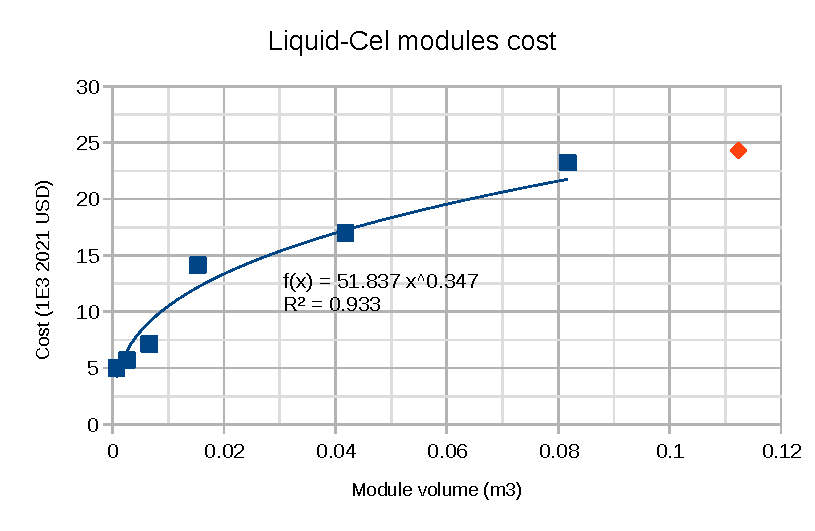
\includegraphics[width=0.6\linewidth, trim={0cm 0cm 0cm 0cm},clip]{MembranesCost.pdf} 
%	\caption{Estimation of Liquid-Cel\textsuperscript{\texttrademark} 14x40 membrane module cost.}
%	\label{fig:MembranesCost}
%\end{figure}

\begin{table}[h] 
\centering
\caption{Liquid-Cel\textsuperscript{\texttrademark} membranes size and cost \protect\citep{LiquidCelData, SGProjects, DPCWaterSolutions}.} \label{table:LiquidCelData}
\resizebox{\columnwidth}{!}{
%	\begin{threeparttable}
\begin{tabular}{@{}ccccc@{}}
	\toprule
	Membrane model & Flow capacity (m3/h) & Diameter (m) & Lenght (m) & Cost (USD) \\ \midrule
	2.5×8          & 0.1 - 0.7            & 0.067        & 0.200      & 5,000       \\
	4×13           & 0.5 - 3.4            & 0.116        & 0.242      & 5,700       \\
	8x20           & 1 - 11               & 0.219        & 0.406      & 14,150      \\
	10x28          & 10 - 48              & 0.279        & 0.683      & 17,000      \\
	%		14x28          & 16 - 91              & 0.356        & 0.821      & 23,200      \\
	14x40          & 16 - 125             & 0.356        & 1.129      & 24,300      \\ \bottomrule
\end{tabular}}
\end{table}

%\begin{table}[h] 
%	\centering
%	\caption{Main characteristics of Liquid-Cel \textsuperscript{\texttrademark} membrane \protect\citep{rongwong2020, ulbricht2013ammonia}.} \label{table:membrane_characteristichs}
%	%	\begin{threeparttable}
	%	\begin{tabular}{@{}cccc@{}}
		%		\toprule
		%		Membrane parameters  & Unit & Variable & Values  \\ \midrule
		%		Number of fibers     & $\frac{\text{fibers}}{\text{m}^2_{\text{module}}}$    & $n_f$       & $2.13 \cdot 10^6$    \\
		%		Fiber outer diameter & m    & $d_o$       & $300 \cdot 10^{-6}$  \\
		%		Fiber inner diameter & m    & $d_i$       & $240 \cdot 10^{-6}$  \\
		%		Pore diameter        & m    & $a$         & $0.04 \cdot 10^{-6}$ \\
		%		Porosity             & -    & $\varepsilon$  & 0.40     \\
		%		Tortuosity factor    & -    & $\tau$      & 2.60     \\
		%		Pressure drop shell side    & bar    & $\Delta P_{\text{shell side}}$      & 0.3     \\
		%		Pressure drop lumen side    & bar    & $\Delta P_{\text{lumen side}}$      & 2     \\
		%		\bottomrule
		%	\end{tabular}
	%\end{table}

Membrane sizing is performed through the membrane mass balances, {\color{blue}{Eqs. \ref{eq:Mem1}-\ref{eq:Mem26}.}} They are based on the distribution of ammonia species within the digestate, mass transfer on the digestate, wetted membrane, and non-wetted membrane phases, and the diffusion of ammonia through the membrane. Ammonia diffusion through the membrane is driven by bulk and Knudsen diffusivities, which consider the mean free path of molecules and the pore diameter respectively. Therefore, the cross-sectional area of the lumen and shell sides, as well as the lenght of the membrane are estimated based on mass balances, as shown in {\color{blue}{Eqs. \ref{eq:A_lumen}, \ref{eq:A_shell}, and \ref{eq:Mem27} of the Supplementary Material respectively.}}

%The main parameters for membrane modeling are calculated in {\color{blue}{Eqs. 
		%\ref{eq:Mem1}-\ref{eq:Mem99}
		%of the Supplementary Material}}, 
%including the cross-sectional area of the lumen and shell sides.
%Digestate density ($\rho$) and viscosity ($\mu$) were assumed equal to those of water.
%%Correlations to estimate these parameters are reported by \citet{hsu1997densities}.
%%Ammonia Henry's constant ($H_{\text{NH}_3}$)
%%%and  Knudsen diffusivity 
%%have been taken from \citet{linstrom2001}.
%%%and  \citet{agrahari2012ml} respectively. The correlations for the rest of parameters can be found in \citet{rongwong2020}:
%
%%\begin{align}
	%%& \rho_{\text{water}} \left(\frac{\text{kg}}{\text{m}^3}\right) = (10^3) \cdot \left(0.863559+1.21494 \cdot 10^{-3} \cdot T(\text{K}) - 2.5708 \cdot 10^{-6} \cdot T(\text{K})^2\right) \label{eq:Mem1} 
	%%\\
	%%& \mu_{\text{water}} \left(\frac{\text{kg}}{\text{m} \cdot \text{s}}\right) = (10^{-6}) \cdot \left(\rho \cdot e^{-3.28285+\frac{456.029}{T(\text{K})-154.576}}\right) \label{eq:Mem2} 
	%%\\
	%%& H_{\text{NH}_3} \left(\frac{\text{kmol}}{\text{atm} \cdot \text{m}^3}\right) = 58 \cdot e^{4100 \cdot \left(\frac{1}{T(\text{K})} - \frac{1}{298.15}\right)}
	%%\label{eq:Mem3}
	%%\end{align}
%
%%The cross-sectional area of the lumen area is calculated based on the transverse area of hollow fiber, and the number of fibers in the membrane module, Eq. \ref{eq:A_lumen} . Shell area is calculated as the difference between total and lumen side cross-sectional areas. 
%Velocities of digestate and stripping fluid (i.e., sulfuric acid solution) are computed based on their respective volumetric flow and transverse areas.
%
%%\begin{align}
	%%& n_{f_{\text{module}}} = A_{\text{module}} \cdot n_f \label{eq:Memnf} 
	%%\\
	%%& A_{\text{lumen side}} \left(\text{m}^2\right) = \frac{d_i^2}{4} \cdot \pi \cdot n_{f_{\text{module}}} \label{eq:A_lumen} 
	%%\\
	%%& A_{\text{shell side}} \left(\text{m}^2\right) = \frac{D_{\text{module}^2}}{4} \cdot \pi - A_{\text{lumen side}} \label{eq:A_shell} 
	%%\\
	%%& V_{\text{stripping fluid}} \left(\frac{\text{m}}{\text{s}}\right) = \frac{\dot{V}_{\text{stripping fluid}}}{A_{\text{lumen side}}} \label{eq:V_stripping}
	%%\\
	%%& V_{\text{digestate}} \left(\frac{\text{m}}{\text{s}}\right) = \frac{\dot{V}_{\text{digestate}}}{A_{\text{shell side}}} \label{eq:V_digestate}
	%%\end{align}
%
%%Diffusion of ammonia through the membrane is driven by bulk and Knudsen diffusivities, which consider the mean free path of molecules and the pore diameter respectively. Bulk diffusivity of ammonia is calculated based on the kinetic theory, using Eq. \ref{eq:Mem5}, while Knudsen diffusivity depends on the molecular velocity, Eq. \ref{eq:Mem4}, and pore diameter, Eq. \ref{eq:Mem7} \citet{agrahari2012ml}. Both contributions to ammonia transport are combined in a effective diffusion coefficient, Eq. \ref{eq:Mem88}. Ammonia diffusion in liquid phase has been assumed equal to ammonia diffusion in water, which is calculated using Eq. \ref{eq:Mem99}. 
%
%The diffusion of ammonia through the membrane is driven by bulk and Knudsen diffusivities, which consider the mean free path of molecules and the pore diameter respectively. Both contributions to ammonia transport are combined in a effective diffusion coefficient, as shown in Eq. \ref{eq:Mem88Manuscript}. Bulk diffusivity of ammonia is calculated based on the kinetic theory,
%%using Eq. \ref{eq:Mem5}, 
%while Knudsen diffusivity depends on the molecular velocity
%%, Eq. \ref{eq:Mem4}, 
%and pore diameter, as shown in {\color{blue}{Eqs. \ref{eq:Mem5} to \ref{eq:Mem99} of the Supplementary Material}}
%%, Eq. \ref{eq:Mem7}
%\citep{agrahari2012ml}.
%%Both contributions to ammonia transport are combined in a effective diffusion coefficient, Eq. \ref{eq:Mem88Manuscript}. Ammonia diffusion in liquid phase has been assumed equal to ammonia diffusion in water, which is calculated using Eq. \ref{eq:Mem99Manuscript}. 
%
%\begin{align}
	%%& \bar{v}  \left(\frac{\text{m}}{\text{s}}\right) = \left(\frac{8 \cdot R\left(\frac{\text{J}}{\text{mol} \cdot \text{K}}\right) \cdot T\left(\text{K}\right)}{MW_{\text{NH}_3} \left(\frac{\text{kg}}{\text{mol}}\right) \cdot \pi} \right)^{\sfrac{1}{2}}
	%%\label{eq:Mem4} 
	%%\\
	%%& D_{\text{NH}_{3}}  \left(\frac{\text{m}^2}{\text{s}}\right) = \frac{1}{3} \cdot \lambda \cdot \bar{v}
	%%\label{eq:Mem5} 
	%%\\
	%%& \lambda  \left(\text{m}\right) = \frac{\kappa \left(\frac{\text{J}}{\text{K}}\right) \cdot T\left(\text{K}\right)}{\pi \cdot \sigma_{\text{NH}_3}^2 \left(\text{m}^2\right) \cdot P\left(\text{Pa}\right) \cdot 2^{\sfrac{1}{2}}}
	%%\label{eq:Mem6} 
	%%\\
	%%& D_{\text{NH}_{3_\text{Kn}}} \left(\frac{\text{m}^2}{\text{s}}\right) = \frac{d_{\text{pore}}}{3} \cdot \left(\frac{8 \cdot R\left(\frac{\text{J}}{\text{mol} \cdot \text{K}}\right) \cdot T(\text{K})} {\pi \cdot MW_{\text{NH}_3} \left(\frac{\text{kg}}{\text{mol}}\right)} \right)^{\sfrac{1}{2}}
	%%\label{eq:Mem7}
	%%\\
	%& D_{\text{eff}} \left(\frac{\text{m}^2}{\text{s}}\right) = \frac{1}{\frac{1}{D_{\text{NH}_{3_\text{Kn}}}} + \frac{1}{D_{\text{NH}_{3}}}}
	%\label{eq:Mem88Manuscript}
	%%\\
	%%& D_{\text{NH}_{3_\text{water}}} \left(\frac{\text{m}^2}{\text{s}}\right) = 1.96 \cdot 10^{-9} \cdot \frac{\mu_{\text{water}_{T=298\text{K}}}}{\mu_{\text{water}_{T}}} \cdot \frac{T\left(\text{K}\right)}{298}
	%%\label{eq:Mem99Manuscript}
	%\end{align}
%
%The distribution of ammonia species shown in Eq. \ref{eq:NH3NH4} is calculated at initial conditions based on the pH of the digestate stream being fed through the tube side of the membrane module, which is assumed equal to 11, as shown in Eq. \ref{eq:Mem9Manuscript}.
%% \ref{eq:Mem11Manuscript}-\ref{eq:Mem10Manuscript}.
%
%\begin{align}
	%%&  f_{\text{NH}_3} = \frac{1}{10^{\left(pK_{a_{\text{NH}_3}}-pH\right)}+1} \label{eq:Mem8} 
	%%\\
	%%&  pK_{a_{\text{NH}_3}} \left(\frac{\text{kmol}}{\text{m}^3}\right) = 0.0901821+\frac{2729.92}{T(\text{K})} \label{eq:Mem11Manuscript} 
	%%\\
	%%&  \left[{\text{NH}_3}\right] = \left[{\text{N}_\text{inorg}}\right] \cdot f_{\text{NH}_3} \label{eq:Mem9} 
	%&  \left[{\text{NH}_3}\right] = \left[{\text{N}_\text{inorg}}\right] \cdot \frac{1}{10^{\left(pK_{a_{\text{NH}_3}}-pH\right)}+1} \label{eq:Mem9Manuscript} 
	%%\\
	%%&  \left[{\text{NH}_4^+}\right] = \left[{\text{N}_\text{inorg}}\right] \cdot \left(1-\frac{1}{10^{\left(pK_{a_{\text{NH}_3}}-pH\right)}+1}\right) \label{eq:Mem10Manuscript} 
	%%&  \left[{\text{NH}_4^+}\right] = \left[{\text{N}_\text{inorg}}\right] \cdot \left(1-f_{\text{NH}_3}\right) \label{eq:Mem10}
	%%\\
	%%&  \left[{\text{H}^+}\right] = K_a \cdot \frac{\left[{\text{NH}_4^+}\right]}{\left[{\text{NH}_3}\right]} \label{eq:Mem12} 
	%\end{align}
%
%%A modified Henry's constant considering the speciation of ammonia is used in the model proposed by \citet{rongwong2020} to evaluate the liquid-solid equilibrium of ammonia, Eq. \ref{eq:Mem13Manuscript}.
%%
%%\begin{align}
	%%&  H_{\text{NH}_3}^* = H_{\text{NH}_3} \cdot \left(1+\frac{K_a \cdot \left[{\text{H}^+}\right]}{Kw}\right) \label{eq:Mem13Manuscript}  
	%%\end{align}
%
%The mass transfer coefficient of the digestate flowing in the tube side, $k_{\text{digestate}}$, is calculated through the Sherwood number of this stream, Eq. \ref{eq:Mem14Manuscript}.
%%and Eqs. \ref{eq:Mem15} and \ref{eq:Mem16}.
%
%\begin{align}
	%&  \text{Sh}_{\text{digestate}} = \frac{k_{\text{digestate}} \cdot d_i}{D_{\text{NH}_{3_\text{water}}}} = 1.62 \cdot \left(\frac{d_i}{L} \cdot \text{Re}_{\text{digestate}} \cdot \text{Sc}_{\text{digestate}}\right)^{\sfrac{1}{3}} \label{eq:Mem14Manuscript}
	%%\\
	%%&  \text{Re}_{\text{digestate}} = \frac{d_i \cdot \rho_{\text{digestate}} \cdot V_{\text{digestate}}}{\mu_{\text{digestate}}} \label{eq:Mem15}
	%%\\
	%%&  \text{Sc}_{\text{digestate}} = \frac{\mu_{\text{digestate}}}{\rho_{\text{digestate}} \cdot D_{\text{NH}_{3_\text{water}}}} \label{eq:Mem16}
	%\end{align}
%
%%The membrane phase can be divided into non-wetted and wetted membrane sections. Their mass transfers coefficients, $k_M$ and $k_M^{'}$ respectively, are calculated based on the fraction of membrane wetted by the digestate. This is calculated based on a correlation reported by \citet{rongwong2020}, shown in Eq. \ref{eq:Mem20}. Eqs. \ref{eq:Mem17}-\ref{eq:Mem18} and \ref{eq:Mem21}-\ref{eq:Mem22} shown the equations employed for the estimation of $k_M$ and $k_M^{'}$ respectively.
%%\begin{align}
	%%& w_{\text{membrane}} = \frac{0.368}{2.709 + e^{-17.486 \cdot \left(V_{\text{digestate}}-0.25\right)}} \label{eq:Mem20}
	%%\\
	%%& d_{\text{interfacial}} \left(\text{m}\right) = d_i + w_{\text{membrane}} \cdot \left(d_o-d_i\right) \label{eq:Mem19}
	%%\\
	%%&  k_M \left(\frac{\text{m}}{\text{s}}\right) = \frac{D_{\text{eff}} \cdot \varepsilon}{\tau \cdot \delta_{\text{non-wetted}}} \label{eq:Mem17}
	%%\\
	%%& \delta_{\text{non-wetted}} \left(\text{m}\right) = \frac{d_o-d_{\text{interfacial}}}{2} \label{eq:Mem18}
	%%\\
	%%&  k_M^{'} \left(\frac{\text{m}}{\text{s}}\right) = \frac{D_{\text{water}} \cdot \varepsilon}{\tau \cdot \delta_{\text{wetted}}} \label{eq:Mem21}
	%%\\
	%%& \delta_{\text{wetted}} \left(\text{m}\right) = \frac{d_{\text{interfacial}}-d_i}{2} \label{eq:Mem22}
	%%\end{align}
%
%%The overall mass transfer coefficient is calculated based on the liquid, wetted membrane, and non-wetted membranes mass transfer coefficients, as shown in Eq. \ref{eq:Mem23}. However, high ammonia concentrations result in a decrease of the overall mass transfer \citep{zhu2005}. Therefore, $K_{ov}$ is modified using a correction factor that consider the concentration of ammonia in digestate.
%
%The overall mass transfer coefficient Eq. \ref{eq:Mem23Manuscript} is calculated based on the liquid, wetted membrane, and non-wetted membranes mass transfer coefficients, calculated in {\color{blue}{Eqs. \ref{eq:Mem17} and \ref{eq:Mem21}}}. However, high ammonia concentrations result in a decrease of the overall mass transfer \citep{zhu2005}. Therefore, $K_{ov}$ is modified using a correction factor that consider the concentration of ammonia in digestate, Eq. \ref{eq:KovCorrectedManuscript}.
%
%\begin{align}
	%& K_{ov} \left(\frac{\text{m}}{\text{s}}\right) = \frac{1}{\left(\frac{1}{k_{\text{digestate}} \cdot d_i} + \frac{1}{k_M^{'} \cdot \delta_{\text{ln wetted}}} + \frac{R \left(\frac{\text{atm} \cdot \text{m}^3}{\text{kmol} \cdot \text{K}}\right) \cdot T(\text{K}) \cdot H_{\text{NH}_3}^{*}}{k_M \delta_{\text{ln non-wetted}}}\right) \cdot d_o } \label{eq:Mem23Manuscript}
	%\\
	%& \delta_{\text{ln wetted}} = \frac{d_{\text{interfacial}}-d_i}{\text{ln}\left( \frac{d_{\text{interfacial}}}{d_i}\right)} \label{eq:Mem24Manuscript}
	%\\
	%& \delta_{\text{ln non-wetted}} = \frac{d_o - d_{\text{interfacial}}}{\text{ln}\left( \frac{d_o}{d_{\text{interfacial}}}\right)} \label{eq:Mem25Manuscript}
	%\\
	%& K_{ov_{\text{corrected}}} \left(\frac{\text{m}}{\text{s}}\right) = K_{ov} \cdot \left(1-\frac{0.002728 \cdot \left[\text{NH}_3\right] \left(\frac{\text{mg}}{\text{L}}\right)}{100}\right) \label{eq:KovCorrectedManuscript}
	%\end{align}
%
%%The mass balance along the membrane can be performed considering the mass transfer in an infinitesimal element of the membrane, as shown in Eq. \ref{eq:Mem26}. Due to the excess of sulfuric acid in the lumen side that lead the formation of ammonium sulfate from the ammonia recovered, the concentration of ammonia in the lumen side is assumed negligible. This differential expression can be analytically integrated to estimate the total length of the membrane, Eq. \ref{eq:Mem27}.
%
%The total length of the membrane can be estimated through Eq. \ref{eq:Mem27Manuscript}, which is obtained from The mass balance along the membrane considering the mass transfer in an infinitesimal element of the membrane, shown in Eq. \ref{eq:Mem26}.
%
%\begin{align}
	%%\frac{\dot{n}_{\text{NH}_3}}{dz} &= -n_{f_{\text{module}}} \cdot \pi \cdot d_o \cdot K_{{ov}_\text{corrected}} \cdot \left( \frac{\dot{n}_{\text{NH}_3}}{\dot{V}_{\text{digestate}}} - \frac{ H_{\text{NH}_3}^* \cdot p_{\text{NH}_3}}{\dot{V}_{\text{digestate}}}\right) \nonumber
	%%\\ 
	%%& \approx -n_{f_{\text{module}}} \cdot \pi \cdot d_o \cdot K_{{ov}_\text{corrected}} \cdot \frac{\dot{n}_{\text{NH}_3}}{\dot{V}_{\text{digestate}}} \label{eq:Mem26}
	%%\\
	%& z \left(\text{m}\right) = \text{ln}\left(\frac{\dot{n}_{\text{NH}_{3_{final}}}}{\dot{n}_{\text{NH}_{3_{initial}}}}\right) \cdot \frac{\dot{V}_{\text{digestate}}}{-n_{f_{\text{module}}} \cdot \pi \cdot d_o \cdot K_{{ov}_\text{corrected}}} \label{eq:Mem27Manuscript}
	%\end{align}

One or multiple membrane modules can be needed to achieve the total membrane length $\left( z \right)$ needed to reach a certain efficiency, as shown in Eq. \ref{eq:nserie}. $n_{\text{series}}$ denotes the necessary number of membrane units of length $L_{\text{module}}$ in-series arrangement to achieve the desired recovery efficiency. The length of the different membrane units is reported in Table \ref{table:LiquidCelData}. $n_{\text{parallel}}$ refers to the number of membrane units in-parallel arrangement required to process the waste flow generated at the livestock facility under study based on the processing capacities reported in Table \ref{table:LiquidCelData}. Membrane modules CAPEX is estimated through Eq. \ref{eq:CAPEXmembrane}, assuming a membrane lifetime $\left(t_{\text{module}}\right)$ of 10 years \citep{verrecht2010cost}, and a plant lifetime $\left(t_{\text{plant}}\right)$ of 20 years. The use of sulfuric acid as stripping fluid and membrane cleaning is the main contributor to membrane OPEX, as shown in Eq. \ref{eq:OPEXmembrane}. Membrane cleaning cost $\left(c_{\text{cleaning}}\right)$ is reported to be between 2\% and 25\% of the operating costs \citep{yu2020performance, verrecht2010cost}, for which we assume an average value of 13.5\%. 
Additionally, the cost of the pumps needed for driving the digestate and stripping fluid streams through the membrane modules is considered. Cost estimation of pumps is collected in {\color{blue}{Eqs. \ref{eq:n_pumps} to \ref{eq:pumpsOPEX} of the Supplementary Material.}}

\begin{align}
	& n_{\text{series}} = \ceil*{\frac{z}{L_{\text{module}}}} \label{eq:nserie}
	\\
	& CAPEX_{\text{membranes}} \left(\text{2019 USD}\right)= \left(n_{\text{serie}} \cdot n_{\text{parallel}}\right) \cdot \nonumber \\
	& Cost_{\text{module}} \left(\frac{\text{USD}}{\text{module}}\right) \cdot \frac{t_{\text{plant}}}{t_{\text{module}}} \label{eq:CAPEXmembrane}
	\\
	& OPEX_{\text{membranes}} \left(\frac{\text{2019 USD}}{\text{year}}\right) = \nonumber \\
	& \frac{\dot{m}_{\text{H}_2 \text{SO}_4} \left(\frac{\text{kg}}{\text{s}}\right)}{\rho_{\text{H}_2 \text{SO}_4} \left(\frac{\text{kg}}{\text{m}^3}\right)} \cdot Price_{\text{H}_2 \text{SO}_4} \left(\frac{\text{USD}}{\text{m}^3}\right) \cdot \frac{1}{1-\frac{c_{\text{cleaning}}}{100}} \label{eq:OPEXmembrane}
\end{align}

%Additionally, pumps to drive the digestate and stripping fluid streams are needed. Their cost is estimated using Eqs. \ref{eq:n_pumps} and \ref{eq:pumpsCAPEX}, assuming that the maximum capacity of one single pump $\left(\dot{V}_{\text{pump}_{\text{max}}}\right)$ is 1 $\sfrac{\text{m}^3}{\text{s}}$ \citep{peters2003plant}. Pumps operating cost are estimated through Eqs. \ref{eq:pumpsH} to \ref{eq:pumpsOPEX}, calculating the energy needed to balance the pressure drop of the shell and lumen sides of the membrane, Table \ref{table:membrane_characteristichs}. Pump efficiencies $\left(\eta_{\text{pump}_i}\right)$ of 0.8 are assumed.
%\begin{align}	
	%&
	%n_{\text{pump}_i} = \ceil*{\frac{\dot{V}_i}{\dot{V}_{\text{pump}_{\text{max}}}}} \label{eq:n_pumps}
	%\\
	%& CAPEX_{\text{pumps}_i} \left(\text{2019 USD}\right) =
	%\begin{cases}
		%(-50.387\cdot10^6 \cdot \dot{V}_i^2 + 1.607\cdot10^6 \cdot \dot{V}_i 
		%\\
		%+ 5.127\cdot10^3) \cdot n_{\text{pump}_i} \cdot 1.055 & \text{if } \dot{V}_i \leq 9\cdot10^{-3} \frac{\text{m}^3}{\text{s}}  \\
		%(92.562\cdot10^3\cdot \dot{V}_i^{0.381}) \cdot n_{\text{pump}_i} \cdot 1.055 & \text{if }  \dot{V}_i > 9\cdot10^{-3} \frac{\text{m}^3}{\text{h}}
		%\end{cases} \label{eq:pumpsCAPEX} \\ 
	%& H_i \left(\text{m}\right) = \frac{\Delta P_i \left(\text{Pa}\right)}{\rho \left(\frac{\text{kg}}{\text{m}^3}\right) g\left(\frac{\text{m}}{\text{s}^2}\right)} \label{eq:pumpsH}
	%\\
	%& \dot{W}_{\text{pump}_i} \left(\text{kW}\right) = \frac{g\left(\frac{\text{m}}{\text{s}^2}\right) \cdot H_i \left(\text{m}\right) \cdot \rho \left(\frac{\text{kg}}{\text{m}^3}\right) \cdot \dot{V}_i \left(\frac{\text{m}^3}{\text{s}}\right)}{\eta_{\text{pump}_i}} \label{eq:pumpsPower}
	%\\
	%& OPEX_{\text{pumps}} \left(\frac{\text{2019 USD}}{\text{year}}\right) = \sum_{i} \dot{W}_{\text{pump}_i} \left(\text{kW}\right) \cdot t_{\text{operation}} \left(\text{s}\right) \cdot 3600 \cdot Price_{\text{electricity}}\left(\frac{\text{USD}}{\text{kWh}}\right) \label{eq:pumpsOPEX}
	%\\
	%& \forall \ i  \in \{\text{shellside, lumenside}\} \nonumber 
	%\end{align}

Total capital and operating expenses for the recovery of nitrogen from livestock digestate using a transmembrane chemisorption process result from the sum of membrane and pump costs are described in Eqs \ref{eq:CAPEX_Transmem} and \ref{eq:OPEX_Transmem}.

\begin{align}	
	& CAPEX_{\substack{\text{transmembrane} \\ \text{chemisorption}}}	= CAPEX_{\text{membranes}} + \sum_{\mathclap{\substack{i 
				\in \\
				\{\text{shellside,} \\ 
				\text{lumenside}\}}}} CAPEX_{\text{pumps}_i} \label{eq:CAPEX_Transmem}
	\\
	& OPEX_{\substack{\text{transmembrane} \\ \text{chemisorption}}}	= OPEX_{\text{membranes}} + OPEX_{\text{pumps}} \label{eq:OPEX_Transmem}
\end{align}	


%\paragraph{\textbf{Ammonia evaporation}} \label{section:Digestate dryingNrecovery}

\textbf{Ammonia evaporation:} Nitrogen can be recovered by ammonia evaporation through digestate drying in a belt dryer unit. The operation of a belt dryer unit requires a minimum concentration of solids of 10\% - 12\% \citep{bolzonella2018nutrients}. Therefore, the liquid and solid outlet streams from the solid-liquid separation stage are combined to obtain a stream with the desired solids content. After solids content adjustment, digestate is dried in the belt drier, as shown in Fig \ref{fig:BeltDryerScheme}. This unit drys the digestate over the belt with a stream of hot air crossing the belt through orifices on it. Heat (sensible and latent) is transferred from the hot air to the digestate on the belt
%in the form of sensible heat, devoted 
to increase temperature
%increase, and latent heat, devoted 
%to the evaporation  
%As a result, 
and evaporate
ammonia and a fraction of moisture.
%+are evaporated. 
%Since the amount of ammonia in digestate is significantly lower than moisture, air saturation with water vapor is considered the evaporation limit. It must be noted that the moisture carrying capacity of air (i.e., the saturation point) is a function of temperature. 
%Therefore, mass and energy balances must be performed simultaneously to determine the amount of ammonia and water carried by the air stream, as well as the final temperature of this stream. 
%An ammonia evaporation yield of 80\% has been assumed based on experimental data \citep{awiszus2018ammonia}. 

%\begin{figure}[h]
%	\centering
%	%	\begin{subfigure}[t]{0.5\linewidth}
%	\includegraphics[width=1\linewidth, trim={0cm 0cm 0cm 0cm},clip]{BeltDryerFinal3.pdf} 
%	\caption{Belt dryer scheme.}
%	\label{fig:BeltDryerScheme}
%\end{figure}

The belt dryer model assumes the evaporation of two components in no equilibrium with a continous extraction of the vapour phase \citep{treybal1980mass}.
%, Eq. \ref{eq:BD11} , 
Since the amount of ammonia in digestate is significantly lower than moisture, air saturation with water vapor is considered the evaporation limit. It must be noted that the moisture carrying capacity of air (i.e., the saturation point) is a function of temperature. This requires to solve the mass and energy balances simultaneously, which are reported in the {\color{blue}{Supplementary Material
%, which are simultaneously solved with the mass balances,
Eqs.
%\ref{eq:BD15} and Eqs.\ref{eq:BD1}-
%\ref{eq:BD11Manuscript}-\ref{eq:BD1Manuscript}
shown in Eqs. \ref{eq:BD11}-\ref{eq:BD10}.}}
%The calculation of the different contributions to energy balances are reported in the {\color{blue}{Supplementary Material, Eqs. \ref{eq:BD2} to \ref{eq:BD10}.}}
%\ref{eq:BD10}.
An ammonia removal efficiency $\left(\eta_{\text{belt dryer}}\right)$ of 80\% has been assumed for mass balances calculation
%, Eq. \ref{eq:BD11Manuscript}
\citep{awiszus2018ammonia}.
%respectively. 
%Air saturation by moisture, Eq. \ref{eq:BD13Manuscript}, and ammonia, Eq. \ref{eq:BD15Manuscript}, represent the upper bound to the carry of these compounds in the air stream. 
The assumptions for the modeling of ammonia evaporation by digestate drying are collected in {\color{blue}{the Section \ref{section:DigDryingNRecoveryPaper} of the Supplementary Material}}.
%The amount of ammonia recovered by evaporation is computed through Eq. \ref{eq:BD11}. 
%The following assumptions has been made for the modeling of digestate drying:
%\begin{itemize}
%	\item $c_{p_{\text{digestate}_{\text{in}}}} \approx c_{p_{\text{water}}}$
%	\item $P_{\text{water}} + P_{\text{NH}_3} \approx P_{\text{water}}$
%	\item $T_{\text{out}_{\text{air}}} = T_{\text{out}_{\text{digestate}}}$
%	\item $\alpha = \text{constant}$
%\end{itemize}

%\begin{align}
%%	& \alpha \cdot \text{ln}\frac{\dot{n}_{\text{water}_\text{in}}}{\dot{n}_{\text{water}_\text{out}}} =  \text{ln}\frac{\dot{n}_{\text{NH\textsubscript{3}}_\text{in}}}{\dot{n}_{\text{NH\textsubscript{3}}_\text{out}}} \label{eq:BD11} 
%%	\\
%%	& \alpha =  \frac{Pv_{\text{NH}_3} \left(T\right)}{Pv_{\text{water}} \left(T\right)} \label{eq:BD12} 
%%	\\
%&\dot{m}_{\text{NH}_{3\text{ evap}}} = \dot{m}_{\text{NH}_{3\text{ in}}} \cdot \eta_{\text{belt dryer}}^{\text{NH}_3} \label{eq:BD11Manuscript} 
%\\
%& \frac{\frac{\dot{m}_{\text{water}_\text{evap}}}{MW_{\text{water}}}}{\sum_{j}\frac{\dot{m}_j}{MW_j}} \cdot P_{\text{total}} \leq Pv_{\text{water}} \left(T\right) \label{eq:BD13Manuscript} 
%\\
%%	& P_{\text{water}} =  \dot{n}_{\text{water}_\text{evap}} \cdot P_{\text{total}} \label{eq:BD14} 
%%	\\
%&\frac{\frac{\dot{m}_{\text{NH}_{3\text{ evap}}}}{MW_{\text{NH}_3}}}{\sum_{j}\frac{\dot{m}_j}{MW_j}} \leq Pv_{\text{NH}_3} \left(T\right) \label{eq:BD15Manuscript} 
%\\
%& \forall \ j \ \in \ \{\text{air}, \ \text{H\textsubscript{2}O}, \ \text{NH}_3\} \nonumber
%%\end{align}
%%
%%\begin{align}
%\\
%& \dot{Q}_{\text{Belt Dryer}} = \dot{H}_{\text{latent}} + \dot{H}_{\text{sensible}} = \dot{H}_{\text{air}_{\text{in}}} - \dot{H}_{\text{air}_{\text{out}}} \label{eq:BD1Manuscript} 
%%\\
%%& \dot{H}_{\text{latent}} = \dot{m}_{\text{water}_\text{evap}} \cdot \lambda_{\text{evap}_{\text{water}}}\left(T\right) + \dot{m}_{\text{NH}_{3_\text{evap}}} \cdot \lambda_{\text{evap}_{\text{NH}_3}}\left(T\right) \label{eq:BD2} 
%%\\
%%& \dot{H}_{\text{sensible}} = \dot{H}_{\text{digestate}_\text{out}} - \dot{H}_{\text{digestate}_\text{in}} + \dot{H}_{\text{sensible}_{\text{gases}}} \label{eq:BD3} \\
%%& \dot{H}_{\text{sensible}_{\text{gases}}} = \left( \dot{m}_{\text{water}_\text{evap}} + \dot{m}_{\text{NH}_{3_\text{evap}}} \right) \cdot c_{p_{\text{water (liquid)}}} \cdot T_{\text{air}_\text{out}} \label{eq:BD4} 
%%\\
%%& \dot{H}_{\text{digestate}_{\text{in}}} = \dot{m}_{\text{digestate}_{\text{in}}} \cdot c_{p_{\text{water}}} \cdot \Delta T_{\text{digestate}_\text{in}} \label{eq:BD5} 
%%\\
%%& \dot{H}_{\text{digestate}_{\text{out}}} = \dot{m}_{\text{digestate}_{\text{out}}} \cdot c_{p_{\text{digestate}}} \cdot \Delta T_{\text{digestate}_\text{out}} \label{eq:BD6} 
%%\\
%%& c_{p_{\text{digestate}}} \left(\sfrac{kg}{kJ \cdot K}\right)= 4.19-0.0275 \cdot \left(\frac{\dot{m}_{\text{TS}_{\text{out}}}}{\dot{m}_{\text{digestate}_{\text{out}}}} \cdot 100 \right) \label{eq:BD7} 
%%\\	
%%& \dot{H}_{\text{air}_{\text{in}}} = \dot{m}_{\text{air}} \cdot c_{p_{\text{air}}} \cdot \Delta T_{\text{air}_\text{in}} \label{eq:BD8} 
%%\\	
%%& \dot{H}_{\text{air}_{\text{out}}} = \left(\dot{m}_{\text{air}} \cdot c_{p_{\text{air}}} + \dot{m}_{\text{water}_\text{evap}} \cdot c_{p_{\text{water (gas)}}} + \dot{m}_{\text{NH}_{3_\text{evap}}} \cdot c_{p_{\text{NH\textsubscript{3} (gas)}}} \right) \cdot \Delta T_{\text{air}_\text{out}} \label{eq:BD9} 
%%\\	
%%& \Delta T_i = T_i - T_\text{ref} \ \forall \ i \ \in \ \{\text{air}_\text{in}, \ \text{air}_\text{out},  \ \text{digestate}_\text{in}, \ \text{digestate}_\text{out} \} \label{eq:BD10}
%\end{align}

Gaseous ammonia is further recovered through acidic scrubbing, as described in Section \ref{section:scrubbing}. 

Capital expenses estimation for belt dryer units is based on the energy required for ammonia evaporation.
%digestate drying.
A drying efficiency $\left(\eta_{\text{belt dryer}}\right)$ of 0.6 has been assumed from the experimental work reported by \citet{awiszus2018utilization}. Belt dryer scale-up is based on the correlation proposed by \citet{towler2012chemical}, as shown in Eq. \ref{eq:CAPEXBeltDryer}. The reference values and scale factor used in this correlation are taken from costs and capacities reported by \citet{turley2016assessment}, as well as the maximum belt dryer capacity used to compute the number of dryer units needed $\left(n_{\text{belt dryer}} \right)$ , as shown in Eq. \ref{eq:nBeltDryer}. These data are also used to estimate the scale-up factor, which is estimated equal to 0.7. Belt dryer operating costs are due to electrical consumption, which has been estimated in 0.099 kW of electricity per kW of thermal energy used by the unit, as shown in Eq. \ref{eq:BeltDryerOPEX} \citep{awiszus2018utilization}.

\begin{align}
%	&
%	\frac{\dot{m}_{\text{water}_\text{evap}}}{t_{\text{operation}}}  
%	\\
& \dot{Q}_{\text{belt dryer}}^{\text{real}} = \frac{\dot{Q}_{\text{belt dryer}}\left(\text{kW}\right)}{\eta_{\text{belt dryer}}} \label{eq:QeltDryerReal} 
\\
& n_{\text{belt dryer}} = \ceil*{\frac{\dot{Q}_{\text{belt dryer}}^{\text{real}}\left(\text{kW}\right)}{1000}} \label{eq:nBeltDryer} 
\\
& \dot{Q}_{\text{belt dryer}}^{\text{design}} = \frac{\dot{Q}_{\text{belt dryer}}^{\text{real}}}{n_{\text{belt dryer}}} \label{eq:QeltDryerDesign} 
\\
& CAPEX_{\text{belt dryer}} \left(\text{2019 USD}\right) = \nonumber \\
& \left(n_{\text{belt dryer}} \cdot 214,997 \cdot \left(\frac{\dot{Q}_{\text{belt dryer}}^{\text{design}}\left(\text{kW}\right)}{500}\right)^{0.7}\right) \cdot 1.216 \label{eq:CAPEXBeltDryer} 
\\
& OPEX_{\text{belt dryer}} \left(\frac{\text{2019 USD}}{\text{year}}\right) = n_{\text{belt dryer}} \cdot \dot{Q}_{\text{belt dryer}}^{\text{design}} \left(\text{kW}\right) \cdot 0.099 \left(\frac{\text{kW}_{\text{e}}}{\text{kW}_{\text{t}}}\right) \cdot \label{eq:BeltDryerOPEX}
\\ 
& t_{\text{operation}} \left(\text{s}\right) \cdot 3600 \cdot Price_{\text{electricity}} \left(\frac{\text{USD}}{\text{kWh}}\right)  \nonumber
\end{align}

%\paragraph{\textbf{Stripping in packed tower}} \label{section:StrippingNrecovery}
\textbf{Stripping in packed tower:} Nitrogen recovery by stripping of the liquid digestate is a widely used technique based on the transfer of ammonia from liquid digestate to an air stream. This operation can be performed either in packed towers or in bubble column reactors, see Section \ref{section:bubblestripping}. Gaseous ammonia is further recovered through acidic scrubbing, as described in Section \ref{section:scrubbing}.

Nitrogen recovery using packed tower stripping, illustrated in Figure \ref{fig:ScrubberScheme}, has been modeled using the number of transfer units (NTU) method \citep{Metcalf}. The pressure drop of tower packing is estimated through the correlation proposed by \citet{kister1991predict}, as shown in Eq. \ref{eq:PDrop}. 

%\begin{figure}[h]
%	\centering
%	%	\begin{subfigure}[t]{0.5\linewidth}
%	\includegraphics[width=0.8\linewidth, trim={0cm 0cm 0cm 0cm},clip]{StrippingScrubbing.pdf} 
%	\caption{Stripping and scrubber towers scheme.}
%	\label{fig:ScrubberScheme}
%\end{figure}

\begin{align}
& P \left(\frac{\text{inch water}}{\text{ft}}\right) = 0.115 \cdot \left( F_{P}  \left(\text{ft}^{-1}\right)\right) ^{0.7} \label{eq:PDrop}
\end{align}

The tower diameter is calculated through the tower flooding capacity. A tower flooding capacity correlation considering the packing pressure drop is developed using ALAMO \citep{wilson2017alamo} based on the flooding curves developed by \citet{strigle1994packed}, as shown in Eq. \ref{eq:FloodingALAMO} and Figure \ref{fig:FloodingALAMO}. Two-inch (0.051 m) Intalox packing is considered \citep{strigle1994packed}, which packing factor $\left(F_P\right)$ is assumed to be 
18 ft\textsuperscript{-1}
(59 m\textsuperscript{-1})
\citep{geankoplis2003transport}. The operating line considered, defined as the ratio of gas and liquid volumetric flows, can be computed through Eqs. \ref{eq:FloodingALAMO} to \ref{eq:OpLine},
where $v_G$ denotes the superficial gas velocity in $\left(\frac{\text{ft}}{\text{s}}\right)$, $\rho_G$ the gas density in $\left(\frac{\text{lb}}{\text{ft}^3}\right) $, $\rho_L$ the liquid density in $ \left(\frac{\text{lb}}{\text{ft}^3}\right) $, $\nu$  the kinematic viscosity in $\left(\text{censtokes}\right)$, $G_G$the gas mass velocity in $\left(\frac{\text{lb}}{\text{ft}^2 \cdot \text{s}}\right)$, and $G_L$ the liquid mass velocity in $\left(\frac{\text{lb}}{\text{ft}^2 \cdot \text{s}}\right) $
\citep{strigle1994packed}.
%, defined as the ratio of gas and liquid volumetric flows, is assumed to be 2668 m\textsuperscript{3}\textsubscript{gas}/m\textsuperscript{3}\textsubscript{liquid} \citep{strigle1994packed}.

\begin{figure}[h!]
\centering
%	\begin{subfigure}[t]{0.5\linewidth}
	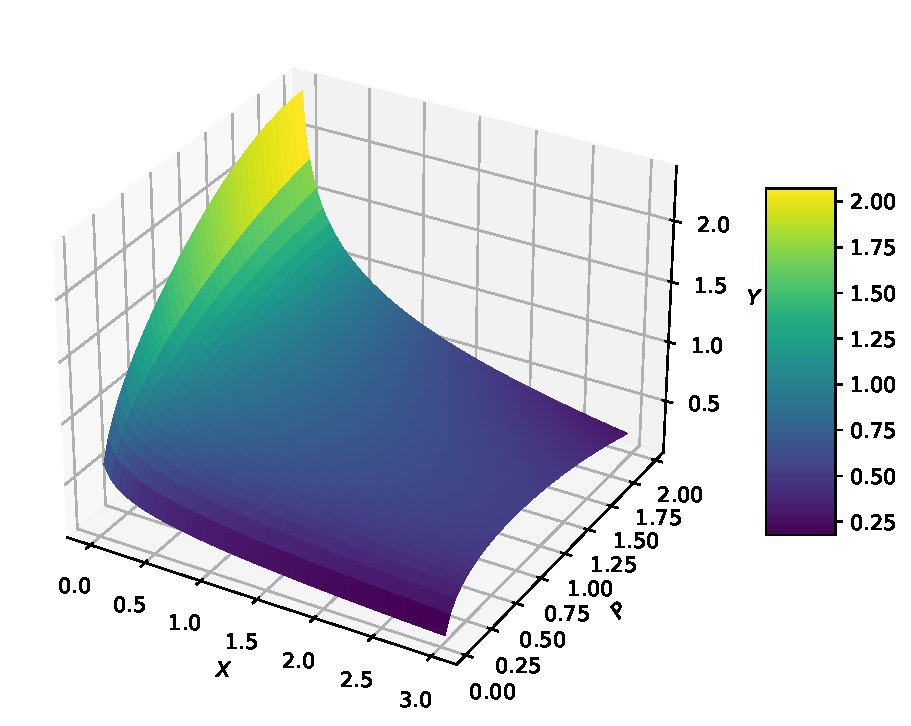
\includegraphics[width=0.72\linewidth, trim={1cm 0cm 0cm 1cm},clip]{gfx/Chapter6/AlamoFlooding.pdf} 
	\caption{Tower flooding capacity correlation considering packing pressure drop.}
	\label{fig:FloodingALAMO}
\end{figure}

%\begin{equation}
	%\begin{split}
		%	Y &=  - 0.25 \cdot X + 0.22 \cdot \text{ln}(P) - 0.78E-01 \cdot P^2 + 0.19E-01 \cdot X^3 - 0.39 \cdot X \cdot P \\
		%	&+ 0.49E-02 \cdot (X\cdot P)^3 + 0.89 \label{eq:FloodingALAMO}
		%\end{split}
	%\end{equation}

\begin{align}
	&Y =  - 0.25 \cdot X + 0.22 \cdot \text{ln}(P) - 0.78\cdot10^{-1} \cdot P^2 + 0.19\cdot10^{-1} \cdot X^3 \nonumber \\
	& - 0.39 \cdot X \cdot P + 0.49\cdot10^{-2} \cdot (X\cdot P)^3 + 0.89 \\
	&Y = v_G \left(\frac{\rho_G}{\rho_L-\rho_G}\right)^{0.5} F_{P}^{0.5} \nu^{0.05} \\
	&X = \text{log}_{10} \left(\frac{G_L}{G_G} \left(\frac{\rho_G}{\rho_L}\right)^{0.5}\right) \\
	&\frac{\dot{V}_G}{\dot{V}_L} = 2688 \ \frac{\text{m}^3_{\text{gas}}}{\text{m}^3_{\text{liquid}}} \label{eq:OpLine}
	%	& P \left(\text{flooding pressure drop}\right) = 0.115 \cdot F_{P}^{0.7} \left(\frac{\text{inch water}}{\text{ft}}\right) \ \left(\text{Empirical equation proposed by Kister and Gill (1991)}\right) \\
	%	& v_G: \text{superficial gas velocity } \left(\frac{\text{ft}}{\text{s}}\right) \\
	%	& \rho_G: \text{gas density} \left(\frac{\text{lb}}{\text{ft}^3}\right) \\
	%	& \rho_L: \text{liquid density} \left(\frac{\text{lb}}{\text{ft}^3}\right) \\
	%	& F_{P}: \text{Packing factor} \left(\text{ft}^{-1} \right); \ F_{P} = 18 \left(\text{ft}^{-1} \right) \ \text{(Geankoplis Table 10.6.1) (2 inch Intalox packing are currently considered for low pressure drop as recommended by Strigle (1987))} \\
	%	& \nu: \text{kinematic viscosity} \left(\text{censtokes}\right); \ \nu = \frac{\mu_L}{\frac{\rho_L}{62.4}} \\
	%	& \mu_L: \text{kinematic viscosity} \left(\text{cP}\right)\\
	%	& 	G_G: \text{gas mass velocity} \left(\frac{\text{lb}}{\text{ft}^2 \cdot \text{s}}\right); \ G_G = v_G \cdot \rho_G \\
	%	& G_L: \text{liquid mass velocity} \left(\frac{\text{lb}}{\text{ft}^2 \cdot \text{s}}\right) 
	\\
	& G_{G_{\text{design}}} = 0.7 G_G = 0.7 \cdot v_G \cdot \rho_G\label{eq:G_Design}
\end{align}

%where:
%
%\begin{itemize}
	%	\item $v_G: \text{superficial gas velocity } \left(\frac{\text{ft}}{\text{s}}\right)$
	%	\item $\rho_G: \text{gas density} \left(\frac{\text{lb}}{\text{ft}^3}\right) $
	%	\item $\rho_L: \text{liquid density} \left(\frac{\text{lb}}{\text{ft}^3}\right) $
	%	\item $F_{P}: \text{packing factor} \left(\text{ft}^{-1} \right)$
	%%	; \ F_{P} = 18 \left(\text{ft}^{-1} \right)$
	%	\item $\nu: \text{kinematic viscosity} \left(\text{censtokes}\right)$
	%%	; \ \nu = \frac{\mu_L}{\frac{\rho_L}{62.4}} $
	%%	\item $\mu_L: \text{kinematic viscosity} \left(\text{cP}\right)$
	%	\item $G_G: \text{gas mass velocity} \left(\frac{\text{lb}}{\text{ft}^2 \cdot \text{s}}\right)$
	%%	; \ G_G = v_G \cdot \rho_G $
	%	\item $G_L: \text{liquid mass velocity} \left(\frac{\text{lb}}{\text{ft}^2 \cdot \text{s}}\right) $
	%\end{itemize}

%\begin{align}
	%	& G_{G_{\text{design}}} = 0.7 G_G = 0.7 \cdot v_G \cdot \rho_G\label{eq:G_Design}
	%\end{align}

The
%theoretical
liquid mass velocity is a known parameter since it corresponds to the digestate being processed. The
%theoretical
gas velocity is estimated by combining Eqs. \ref{eq:PDrop}, \ref{eq:FloodingALAMO}, and \ref{eq:OpLine}. The design gas mass velocity considered is 0.7 time the theoretical gas mass velocity, Eq \ref{eq:G_Design}, while the liquid design mass velocity is computed by combining Eqs. \ref{eq:G_Design} and \ref{eq:OpLine}.
%The tower diameter is computed based on the design liquid mass velocity and liquid mass flow. However, 
Design restrictions reported by \citet{Branan} have been considered in the sizing of the packed tower.
The tower height is estimated through the height and number of transfer units \citep{Metcalf}, as described in the Supplementary Material, Eqs. \ref{eq:HTUStripping} to \ref{eq:Stripping2Ddesign}.

%, Eqs \ref{eq:DRestriction} and \ref{eq:ZRestriction} \citep{Metcalf}. Therefore, the design diameter is computed as shown in Eqs. \ref{eq:A_Stripping} to \ref{eq:StrippingDdesign}. Additionally, the number of packed towers that have to be install in parallel is estimated through Eq. \ref{eq:nStrippers}.

%\begin{align}
	%	&D_{\text{design}} \leq 1.2 \text{ m}  \label{eq:DRestriction}\\
	%	& \frac{H_{\text{design}}}{D_{\text{design}}} \leq 30 \label{eq:ZRestriction}\\
	%	& A_{\text{stripping tower}} = \frac{\dot{m}_L}{G_{L_{\text{design}}}} \label{eq:A_Stripping} \\
	%	& D_{\text{stripping tower}} = \left(\frac{A_{\text{stripping tower}}}{\pi}\right)^{0.5} \label{eq:D_Stripping} \\
	%	& D_{\text{stripping tower}}^{\text{design}} \left(\text{m}\right) =
	%	\begin{cases}
		%		D_{\text{stripping tower}} & \text{if } 	D_{\text{stripping tower}} \leq 1.2 \text{ m}  
		%		\\
		%		1.2 & \text{if }  D_{\text{scrubber}} > 1.2 \text{ m}
		%	\end{cases} \label{eq:StrippingDdesign} \\
	%	& n_{\text{stripping tower}}^{\text{parallel}} = \ceil*{\frac{D_{\text{stripping tower}}(\text{m})}{1.2}}\label{eq:nStrippers}
	%\end{align}
%
%The height of the stripping packed towers is estimated through the height and number of transfer units, Eq. \ref{eq:HTUStripping} and \ref{eq:NTUStripping} respectively \citep{Metcalf}. The liquid overall mass transfer coefficient value assumed for the ammonia air system is 2 h\textsuperscript{-1} \citep{larsen2013source}. The design restriction shown in Eq. \ref{eq:ZRestriction} is considered to compute the design height of the stripping towers, and the number of units that must be installed in series, Eq. \ref{eq:nStrippersSerie}.
%
%\begin{align}
	%	& HTU = \frac{\frac{\dot{m}_L}{n_{\text{stripping tower}}^{\text{parallel}} \cdot\rho_{\text{digestate}}}}{K_{L}a \cdot \pi \cdot \left(\frac{D_{\text{stripping tower}}}{2}\right)^2} \label{eq:HTUStripping} \\
	%	& NTU = \frac{S}{S-1} \text{ln}\left(\frac{\frac{1}{1-\sfrac{\eta_{\text{stripping tower}}}{100}} \cdot \left(S-1\right) + 1}{S}\right) \label{eq:NTUStripping} \\
	%	& S = \frac{H_{\text{NH}_3}}{P_{\text{stripping tower}}} \cdot \frac{\dot{m}_G}{\dot{m}_L} \\
	%	& H_{\text{stripping tower}} = NTU \cdot HTU \label{eq:HStripping} \\
	%	& n_{\text{stripping tower}}^{\text{series}} = \ceil*{\frac{\frac{H_{\text{stripping tower}}}{ D_{\text{stripping tower}}^{\text{design}}}}{30}}\label{eq:nStrippersSerie}\\
	%	& H_{\text{stripping tower}}^{\text{design}} \left(\text{m}\right) =
	%	\begin{cases}
		%		H_{\text{stripping tower}} & \text{if } 	\frac{H_{\text{stripping tower}}}{D_{\text{stripping tower}}} \leq 30  
		%		\\
		%		\frac{\frac{\dot{m}_L}{n_{\text{stripping tower}}^{\text{series}} \cdot n_{\text{stripping tower}}^{\text{parallel}} \cdot\rho_{\text{digestate}}}}{K_{L}a \cdot \pi \cdot \left(\frac{D_{\text{stripping tower}}}{2}\right)^2} & \text{if } 	\frac{H_{\text{stripping tower}}}{D_{\text{stripping tower}}} \leq 30  
		%	\end{cases} \label{eq:Stripping2Ddesign}
	%\end{align}

The number of stripping units needed $\left( n_{\text{stripping tower}} \right) $ is calculated as the product of the number stripping units in-series arrangement to satisfy the packed towers height limit $\left(n_{\text{stripping tower}}^{\text{series}} \right) $ and the number stripping units in-parallel arrangement to process the amount of waste generated in the livestock facility under evaluation $\left( n_{\text{stripping tower}}^{\text{parallel}} \right) $, as shown in Eq. \ref{eq:n_stripping}. CAPEX of stripping packed towers is estimated based on the columns volume using a correlation based on data from CAPCOST \citep{CAPCOST}, as shown Eq. \ref{eq:CAPEXScrubber}. Additionally, capital expenses of compressor units are estimated based on the correlation reported by \citet{almena2016technoeconomic}, Eq. \ref{eq:CAPEXCompressor}. Operating expenses of scrubbing are mainly due to the compression cost, Eq. \ref{eq:compressorOPEX}.

\begin{align}
	& n_{\text{stripping tower}} = n_{\text{stripping tower}}^{\text{series}} \cdot  n_{\text{stripping tower}}^{\text{parallel}} \label{eq:n_stripping} \\
	& CAPEX_{\text{stripping tower}} \left(\text{2019 USD}\right) = 1.216 \ n_{\text{stripping tower}} \cdot  \nonumber
	\\
	& \left(-6.157 \cdot \left(V_{\text{stripping tower}} \left(\text{m}^3\right)\right)^2 + 1276.035 \cdot V_{\text{scrubber}} \left(\text{m}^3\right) + 4007.619\right) \label{eq:CAPEXScrubber}
	\\
	& V_{\text{stripping tower}} = \frac{\left(D_{\text{stripping tower}}^{\text{design}}\right)^2 \cdot \pi}{4} \cdot H_{\text{stripping tower}} 
	\\
	&
	CAPEX_{\text{compressor}} \left(\text{2019 USD}\right) = 1.216 \cdot \nonumber \\
	& \left(335.27 \cdot \dot{W}_{\text{compressor}} \left(\text{kW}\right) + 36211\right) \label{eq:CAPEXCompressor}
	\\
	& OPEX_{\text{compressor}} \left(\frac{\text{2019 USD}}{\text{year}}\right) = \dot{W}_{\text{compressor}} \left(\text{kW}\right) \cdot t_{\text{operation}} \left(\text{s}\right) \cdot \nonumber \\
	& 3600 \cdot Price_{\text{electricity}}\left(\frac{\text{USD}}{\text{kWh}}\right) \label{eq:compressorOPEX}
\end{align}	

%\paragraph{\textbf{{\color{red}{Aerated bubble stripping}}}}\label{section:bubblestripping}

%\paragraph{\textbf{Acidic scrubbing}} \label{section:scrubbing}
\textbf{Acidic scrubbing:} Ammonia contained in the gaseous streams from
%digestate drying
ammonia evaporation
%(described in Section \ref{section:Digestate dryingNrecovery})
and stripping in packed bed
%(described in Section \ref{section:StrippingNrecovery})
can be recovered in an acidic scrubbing stage using a solution of sulfuric acid in water, as described in Fig. \ref{fig:ScrubberScheme}. Ammonia is trapped by the liquid stream, reacting with the sulfuric acid to form ammonium sulfate.
%{\color{red}{This is a solid element that can be recovered by sedimentation or filtration}}. 
Mass balances for the scrubber unit consider the water transferred to the gas stream, assuming that saturation is reached, Eq. \ref{eq:SC2}. Ammonia  recovery efficiency ($\eta_{scrubber}^{\text{NH}_3}$) of full-scale ammonia scrubbers has been reported in the range of 40\% to 99\% \citep{melse2005}. A typical $\eta_{scrubber}^{\text{NH}_3}$ of 96\% has been selected based on the work of \citet{melse2005}.

%\begin{figure}[H]
%	\centering
%	%	\begin{subfigure}[t]{0.5\linewidth}
%	\includegraphics[width=0.8\linewidth, trim={0cm 0cm 0cm 0cm},clip]{StrippingScrubbing.pdf} 
%	\caption{Stripping and scrubber towers scheme.}
%	\label{fig:ScrubberScheme}
%\end{figure}

\begin{align}
& \frac{P_{\text{water}}}{Pv_{\text{water}}} = 1 \label{eq:SC1} 
\\
& Pv_{\text{water}} = \frac{\frac{\dot{m}_{\text{water}_{out}}^{\text{gas stream}}}{MW_\text{water}}}
{\sum_{j}\frac{\dot{m}_{\text{j}}^{\text{gas stream}}}{MW_\text{j}}}
\cdot P_{in}^{\text{gas stream}} \label{eq:SC2} 
\\
& \dot{m}_{\text{NH}_{3 \ out}}^{\text{gas stream}} = \dot{m}_{\text{NH}_{3 \ in}}^{\text{gas stream}} \cdot \left(1-\eta_{scrubber}^{\text{NH}_3}\right) \label{eq:SC3}
\end{align}

The water flow needed to perform the scrubbing operation is computed from the operation line of the unit $\left(\sfrac{L}{G}\right)$, Eq. \ref{eq:SC4}. Following the rules of thumb for scrubbing units, the design operation line has been assumed as twice the minimum operation line, Eq. \ref{eq:SC5}. $Y_{\text{NH}_3}$ and $X_{\text{NH}_3}$ denote the ammonia free basis molar fractions in gas and liquid streams respectively. The amount of sulfuric acid supplied to make-up the sulfate used for ammonium sulfate formation, Eq. \ref{eq:SC7}, is slightly larger than the stoichiometric amount of the precipitation reaction, 3.5 $\text{kg}_{\text{H}_2 \text{SO}_4}$ per ${\text{kg}_{\text{NH}_3}}$ recovered \citep{bolzonella2018nutrients}.

\begin{align}
& \left(\sfrac{L}{G}\right)_{\text{min}}= \frac{Y_{\text{NH}_{3 in}} - Y_{\text{NH}_{3 out}}}{X_{\text{NH}_{3 out}} - X_{\text{NH}_{3 in}}} \label{eq:SC4} 
\\
& \left(\sfrac{L}{G}\right)= \left(\sfrac{L}{G}\right)_{\text{min}} \cdot 2 \label{eq:SC5} 
\\
& \dot{m}_{\text{water}_{in}}^{\text{liquid stream}} = \left(\left(\sfrac{L}{G}\right) \cdot \dot{n}_{\text{total}_{in}}^{\text{liquid stream}} - \dot{n}_{\text{NH}_{3 \ in}}^{\text{liquid stream}}\right) \cdot MW_{\text{water}} \label{eq:SC6} 
\\
& \dot{m}_{\text{H}_2 \text{SO}_{4_{in}}}^{\text{liquid stream}} = \dot{m}_{\text{NH}_{3 \ in}}^{\text{gas stream}} \cdot \eta_{scrubber}^{\text{NH}_3} \cdot 3.5 \label{eq:SC7} 
\\
& \dot{m}_{\left(\text{NH}_4\right)_2 \text{SO}_{4_{out}}}^{\text{liquid stream}} = \frac{\dot{m}_{\text{NH}_{3 \ in}}^{\text{gas stream}} \cdot \eta_{scrubber}^{\text{NH}_3}}{MW_{\text{NH}_3}} \cdot MW_{\left(\text{NH}_4\right)_2 \text{SO}_{4_{out}}} \label{eq:SC8} 
\end{align}

Scrubbing CAPEX is estimated through a preliminary design and sizing of the scrubbing units. As shown in the {\color{blue}{Section \ref{section:AcidicScrubbingNRecoveryPaper} of the Supplementary Material,}} the estimation of the scrubber diameter is based on the gas velocity in the equipment \citep{melse2005}. The number of units is set by the maximum diameter of scrubbers, Eq. \ref{eq:nscrubbers}, which is assumed equal to 1.2 m accordingly to the rules of thumb for packed columns \citep{Branan}. Similarly to the case of stripping columns, the height of scrubbing towers is computed through the transfer units method, as described by \citet{couper2005chemical}. This method is shown in {\color{blue}{ Eqs. \ref{eq:Hscrubber}-\ref{eq:HTU} of the Supplementary Material.}}

%The scrubber diameter, Eq. \ref{eq:scrubberDdesign}, is based on the gas velocity in the equipment, which is assumed equal to 1.75 $\sfrac{\text{m}}{\text{s}}$ \citep{melse2005}. The number of units is set by the maximum diameter of scrubbers, Eq. \ref{eq:nscrubbers}, which is assumed equal to 1.2 m accordingly to the rules thumb for packed columns \citep{Branan}.
%
%\begin{align}	
%& D_{\text{scrubber}} \left(\text{m}\right) = \frac{\dot{V}^{\text{gas stream}} \left(\frac{\text{m}^3}{\text{s}}\right)}{1.75 \left(\frac{\text{m}}{\text{s}}\right)} \label{eq:scrubberD}
%\\
%& D_{\text{scrubber}}^{\text{design}} \left(\text{m}\right) =
%\begin{cases}
	%D_{\text{scrubber}} & \text{if } 	D_{\text{scrubber}} \leq 1.2 \text{ m}  
	%\\
	%1.2 & \text{if }  D_{\text{scrubber}} > 1.2 \text{ m}
	%\end{cases} \label{eq:scrubberDdesign} \\
%& n_{\text{scrubbers}} = \ceil*{\frac{\dot{V}^{\text{gas stream}} \left(\frac{\text{m}^3}{\text{s}}\right)}{1.75 \left(\frac{\text{m}}{\text{s}}\right) \cdot \frac{1.2^2 \left(\text{m}^2\right)}{4} \pi }}\label{eq:nscrubbers}
%\end{align}	

%The height of scrubbing units is estimated through the height and number of transfer units, Eq. \ref{eq:Hscrubber}, as described by \citet{couper2005chemical}. The number of transfer units is determined by the Kremser shortcut method, as shown in Eq. \ref{eq:Kremser} \citep{seader2004product}, while the height of each transfer unit is calculated in Eq. \ref{eq:HTU}. The gas film overall mass transfer coefficient value for the ammonia air system is 272474.56 $\frac{\text{mol}}{\text{h·m\textsuperscript{3}·atm}}$ \citep{Branan}. 
%The scrubbing operation involve the use of compressors for pumping the stripping gas stream. The energy required for compression is estimated through {\color{blue}{Eq. \ref{eq:CompressorEnergy} of the Supplementary Material.}}
%%  Fig. \ref{fig:vessel_investment_cost}.
%
%\begin{align}	
%%	&
%%	x_{\text{NH}_{3 in}}^{\text{gas stream}} = \frac{\dot{n}_{\text{NH}_{3 in}}^{\text{gas stream}}}{\dot{n}^{\text{gas stream}}}
%%	\\
%%	&
%%	x_{\text{NH}_{3 out}}^{\text{gas stream}} = \frac{\dot{n}_{\text{NH}_{3 out}}^{\text{gas stream}}}{\dot{n}^{\text{gas stream}}}
%%	\\
%& H_{\text{scrubber}} = NTU \cdot HTU \label{eq:Hscrubber}
%\\
%& NTU = \frac{\text{ln}\left(\left(1-m \cdot \frac{\dot{n}^{\text{gas stream}}}{\dot{n}^{\text{liquid stream}}} \right) \frac{x_{\text{NH}_{3 in}}^{\text{gas stream}} - x^*_{\text{NH}_{3}}}{x_{\text{NH}_{3 out}}^{\text{gas stream}} - x^*_{\text{NH}_{3}}} + m \cdot\frac{\dot{n}^{\text{gas stream}}}{\dot{n}^{\text{liquid stream}}}\right)}{\text{ln}\left(m \cdot \frac{L}{V}\right)}\label{eq:Kremser}
%\\
%&
%x_{\text{NH}_{3 k}}^{\text{gas stream}} = \frac{\dot{n}_{\text{NH}_{3 k}}^{\text{gas stream}}}{\dot{n}^{\text{gas stream}}}, \ \forall \ k \ \in \ \{in, out\}
%\\
%&
%x^*_{\text{NH}_{3}} = 0
%\\
%&
%m = \frac{P_{\text{NH}_3}}{P}
%\\
%& HTU = \frac{\dot{n}^{\text{gas stream}} \left(\frac{\text{mol}}{\text{h}}\right)}{\pi \cdot \frac{D_{\text{scrubber}}^{\text{design}^2}}{4} \left(\text{m}^2\right)\cdot k_{GA} \left(\frac{\text{mol}}{\text{h·m\textsuperscript{3}·atm}}\right)\cdot P \left(\text{atm}\right)}\label{eq:HTU}
%\end{align}

%The scrubbing operation involve the use of compressors for pumping the stripping gas stream. The energy required for compression is estimated though Eq. \ref{eq:CompressorEnergy}, assuming a compressor efficiency $\left(\eta_{\text{compressor}}\right)$ of 0.85 and a polytropic coefficient $\left(k\right)$ of 1.4. The pressure drop of a typical scrubber for ammonia capture assumed is 200 Pa \citep{melse2005}.
%
%\begin{align}
%\dot{W}_{\text{compressor}} \left(\text{kW}\right) = \frac{k \cdot R \left(\frac{\text{J}}{\text{K} \cdot \text{kmol}}\right) \cdot T_{in}^{\text{gas stream}} \left(\text{K}\right) \cdot \dot{m}_{in}^{\text{gas stream}} \left(\frac{\text{kg}}{\text{s}}\right)}{\eta_{\text{compressor}} \cdot \left(k-1\right) \cdot MW_{gas}} \cdot \left(\left(\frac{P_{in}^{\text{gas stream}}}{P_{out}^{\text{gas stream}}}\right)^{\frac{k-1}{k}}-1\right) \label{eq:CompressorEnergy}
%\end{align}

%CAPEX of scrubber units is estimated based on the columns volume using a correlation based on data from CAPCOST \citep{CAPCOST}, Eq. \ref{eq:CAPEXScrubber}. Additionally, capital expenses of compressor units are considered, Eq. \ref{eq:CAPEXCompressor}. 
CAPEX of scrubber units is estimated through the column's volume by using the correlation described in Eq. \ref{eq:CAPEXScrubber}. The cost of the compressor is estimated through Eq. \ref{eq:CAPEXCompressor}.
Operating expenses of scrubbing are mainly related to the use of sulfuric acid, Eq. \ref{eq:OPEXScrubber}, and the compression cost, Eq. \ref{eq:compressorOPEX2}.

\begin{align}
%& CAPEX_{\text{scrubbers}} \left(\text{2019 USD}\right) = 1.216 \ n_{\text{scrubbers}} \cdot  \nonumber
%\\
%& \left(-6.157 \cdot \left(V_{\text{scrubber}} \left(\text{m}^3\right)\right)^2 + 1276.035 \cdot V_{\text{scrubber}} \left(\text{m}^3\right) + 4007.619\right) \label{eq:CAPEXScrubber}
%\\
%& V_{\text{scrubber}} = \frac{\left(D_{\text{scrubber}}^{\text{design}}\right)^2 \cdot \pi}{4} \cdot H_{\text{scrubber}} 
%\\
%&
%CAPEX_{\text{compressor}} \left(\text{2019 USD}\right) = 1.216 \cdot \left(335.27 \cdot \dot{W}_{\text{compressor}} \left(\text{kW}\right) + 36211\right) \label{eq:CAPEXCompressor}
%\\
& OPEX_{\text{scrubbers}} \left(\frac{\text{2019 USD}}{\text{year}}\right) = \frac{\dot{m}_{\text{H}_2 \text{SO}_4} \left(\frac{\text{kg}}{\text{s}}\right)}{\rho_{\text{H}_2 \text{SO}_4} \left(\frac{\text{kg}}{\text{m}^3}\right)} \cdot Price_{\text{H}_2 \text{SO}_4} \left(\frac{\text{USD}}{\text{m}^3}\right)  \label{eq:OPEXScrubber}
\\
& OPEX_{\text{compressor}} \left(\frac{\text{2019 USD}}{\text{year}}\right) = \dot{W}_{\text{compressor}} \left(\text{kW}\right) \cdot t_{\text{operation}} \left(\text{s}\right) \cdot \nonumber \\
& 3600 \cdot Price_{\text{electricity}}\left(\frac{\text{USD}}{\text{kWh}}\right) \label{eq:compressorOPEX2}
\end{align}	

%Total CAPEX and OPEX for nitrogen recovery though digestate drying are calculated in Eqs. \ref{eq:CAPEXDigDrying} and \ref{eq:OPEXDigDrying}.
%
%\begin{align}
%& CAPEX_{\text{digestate drying}} = \sum_{k}  CAPEX_k  \label{eq:CAPEXDigDrying}
%\\
%& OPEX_{\text{digestate drying}} = \sum_{k}  OPEX_k \label{eq:OPEXDigDrying}
%\\
%& \forall \ k \ \in \ \{\text{belt dryer}, \text{scrubbers}, \text{compressor}\} \nonumber
%\end{align}


%\begin{figure}[H]
%	\centering
%	%	\begin{subfigure}[t]{0.5\linewidth}
	%	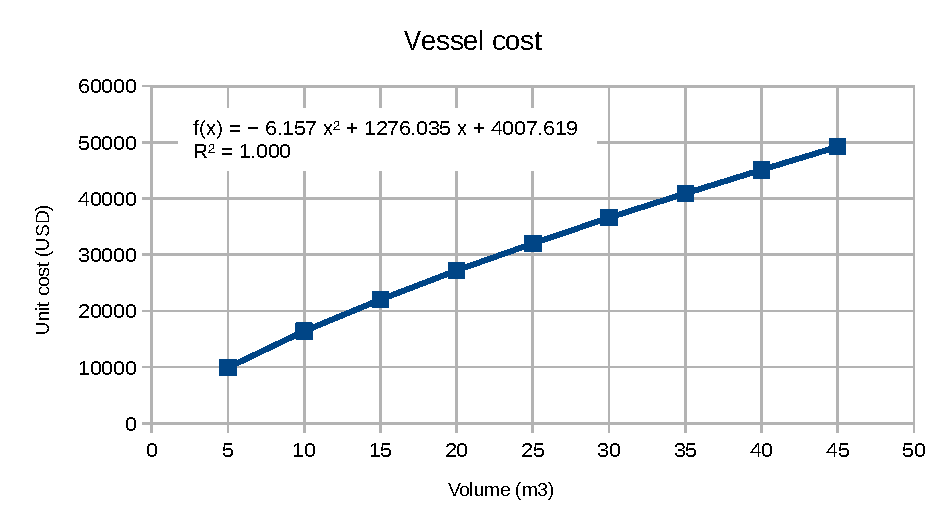
\includegraphics[width=0.7\linewidth, trim={0cm 0cm 0cm 0cm},clip]{vessel_investment_cost.pdf} 
	%	\caption{Estimated investment costs for a non-jacketed vessel, based on data from CAPCOST \protect\citep{CAPCOST}.}
	%	\label{fig:vessel_investment_cost}
	%\end{figure}

%\paragraph{Stripping}
%{\color{red}{Not done yet}}
%
%\paragraph{Ultrafintration and reverse osmosis}
%{\color{red}{Under consideration}}

\subsection{Economic assessment}

%{\color{red}{OJO Neither uncertaininty}}

The total costs of nitrogen recovery and waste processing have been estimated for each nitrogen management system evaluated. These are defined in Eqs. \ref{eq:NRecCost} and \ref{eq:WasteProcCost} respectively for each evaluated technology $i$, where $k$ represents the possible products obtained, $i$ denotes the discount rate (assumed to be 7\%), and $n_{\text{plant}}$ represents the process lifetime, which is assumed to be 20 years. Cost estimation includes OPEX and CAPEX amortization of all equipment involved in the processing of swine waste, as well as incomes from the sale of recovered products for those processes producing struvite (Multiform) or ammonium sulphate (digestate drying, stripping in packed tower, and membrane system). 
%CAPEX and OPEX of the systems evalauted are shown in the {\color{blue}{Supplementary Material, Figure 1S}}. 
The selling prices considered are 0.85 USD per kilogram of struvite \citep{molinos2011economic}, and 0.12 USD per kilogram of ammonium sulphate \citep{AmmoniumSulphatePrice}. Conversely, the liquid and organic solid effluents containing low concentrations of nitrogen, such as the products obtained from the MAPHEX system, as well as some streams recovered from other systems such as ammonia evaporation or struvite production, are considered products with no market value. This assumption is based in the fact that, although they can be used for nutrient supplementation in croplands, they are too bulky for being economically transported to nutrient deficient areas. Therefore, similarly to manure, they can just be applied locally, hindering their use as a bio-based substitute of synthetic nitrogen fertilizers.
%The product recovered form MAPHEX system is a solid mainly comprised of organic matter, containing nutrients such as nitrogen and phosphorus. However, since the concentration of nutrients in this material is much lower than struvite or ammonium sulfate, hindering the transportation of this solid, it has been assumed that no incomes can be obtained from this product.

\begin{align}
& Cost_{j}^{\substack{nitrogen\\recovery}} \left(\frac{\text{USD}}{\text{kg\textsubscript{N recovered}}}\right) = \nonumber \\
& \frac{OPEX_{j}+CAPEX_{j} \cdot \frac{i \cdot \left( \left(1+i\right)^{n_{\text{plant}}} \right)}{\left( \left( 1+i\right)^{n_{\text{plant}}} -1 \right) } -\sum_{k}{\dot{m}_{j,k} \cdot Price_{k}}}{{\dot{m}_{N_{recovered}}}} \label{eq:NRecCost} \\
\nonumber \\
& Cost_{j}^ {\substack{waste\\processing}} \left(\frac{\text{USD}}{\text{kg\textsubscript{Waste processed}}}\right) = \nonumber \\
& \frac{OPEX_{j}+CAPEX_{j} \cdot \frac{i \cdot \left( \left(1+i\right)^{n_{\text{plant}}} \right)}{\left( \left( 1+i\right)^{n_{\text{plant}}} -1 \right) } -\sum_{k}{\dot{m}_{j,k} \cdot Price_{k}}}{\dot{m}_{Waste_{processed}}} \label{eq:WasteProcCost}
\end{align}

%\subsection{Nitrogen releases environmental geographic information system framework}


\section{Results and discussion}
\subsection{Nitrogen flows and recovery efficiency}
%The nitrogen recovery efficiency of the evaluated systems is shown in Figure \ref{fig:N_recovery_techs}. The efficiencies are reported considering both the entire process of waste treatment (including waste pretreatment and N recovery) and the technology for nitrogen recovery only. This approach is used in order to compare not just the technologies used for the recovery of nitrogen, but also the pretreatment stages required by each system for the recovery of nitrogen from swine waste. Therefore, the recovery efficiency considering the whole process represents the actual fraction of nitrogen recovered, while the efficiency of each technology only represents the nitrogen recovered after waste conditioning. 
%
%\begin{figure}[H]
%	\centering
%	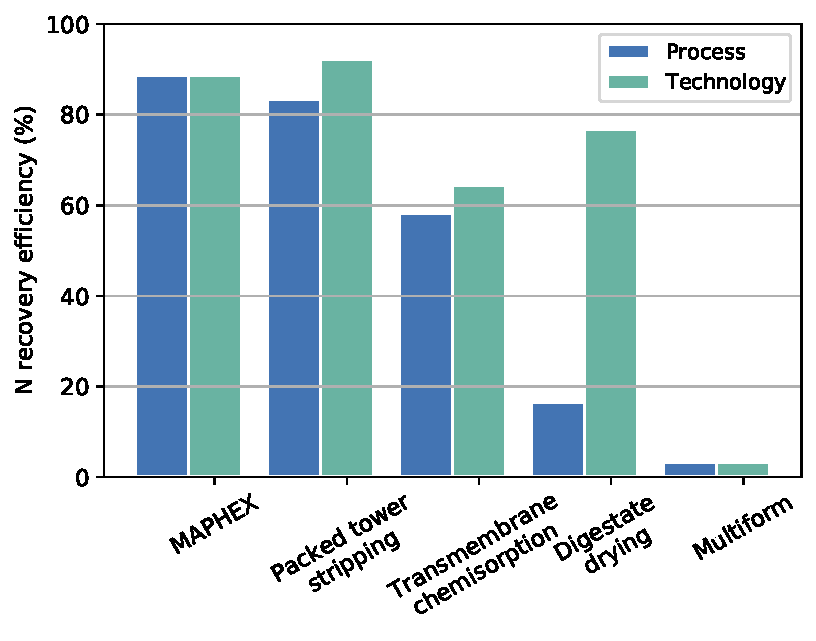
\includegraphics[angle=0, width=0.6\textwidth, trim={0cm 0cm 0cm 0cm}, clip]{N_recovery_techs.pdf}
%	\caption{Nitrogen recovery efficiency considering only nutrient recovery technologies and the entire waste treatment process. The recovery efficiency considering the whole process represents the actual fraction of nitrogen recovered.}
%	\label{fig:N_recovery_techs}
%\end{figure}

The nitrogen flows of the evaluated systems have been analyzed to determine the fraction of nitrogen recovered as inorganic products, either in the form of ammonium sulphate solution or as struvite, the the nitrogen recovered within the organic solid fraction of the waste, and the fraction of nitrogen that it is not recovered and is released into the environment, as shown in Figure \ref{fig:Sankeys}. The nitrogen flows have been analyzed considering the entire recovery systems for waste treatment, including the pretreatment and N recovery processes.

It can be observed that the
%digestate drying
ammonia evaporation process
%is performed through evaporation of the ammonia contained in digestate using a belt dryer. However, this process
requires a waste stream with a high solids content for the ammonia evaporation in the belt dryer unit.
% of digestate, 
Therefore, a solid adjustment must be performed, 
%resulting in low recovery efficiencies due to the
discarding a large fraction of the liquid phase of digestate, which contains most of the inorganic nitrogen. As a result, a significant fraction of nitrogen (79 \%) is released in a liquid stream. Nitrogen recovery by stripping in packed tower and membrane systems results in a fraction of nitrogen recovered in the organic solid fraction of the waste as a consequence of liquid-solid separation stages, in addition to the nitrogen recovered as a solution of ammonium sulphate, as illustrated in Figures \ref{fig:NitrogenFlow_StrippingPacked_sankey} and \ref{fig:NitrogenFlow_Membrane_sankey}. 

%On the other hand, the low recovery efficiency of 
Multiform system show a low efficiency of nitrogen recovered as struvite. This is due to the fact that phosphate is the limiting factor for stuvite production, since this compound is in much lower concentrations than nitrogen in swine waste, as reported in Table \ref{table:SwineWaste}. As a result, a significant fraction of nitrogen is not recovered but released in a liquid stream, similarly to ammonia evaporation process, as observed in \ref{fig:NitrogenFlow_MULTIFORM_sankey}.
%is mainly due to the struvite precipitation rather than waste pretreatment, as observed in \ref{fig:NitrogenFlow_MULTIFORM_sankey}. The presence of phosphate is the limiting factor for stuvite production, since this compound is in much lower concentrations than nitrogen in swine waste, as reported in Table \ref{table:SwineWaste}. 
Finally, since MAPHEX is a manure processing system that integrates all the stages from the feed of raw manure to the recovery of the final products, no pretreatment stages are considered for this system. The nitrogen is recovered within a organic solid material, as shown in Figure \ref{fig:NitrogenFlow_MAPHEX_sankey}. 

%\begin{sidewaysfigure}
\begin{figure}[h!]
	\centering
	\begin{subfigure}[t]{0.99\textwidth}
		\centering
		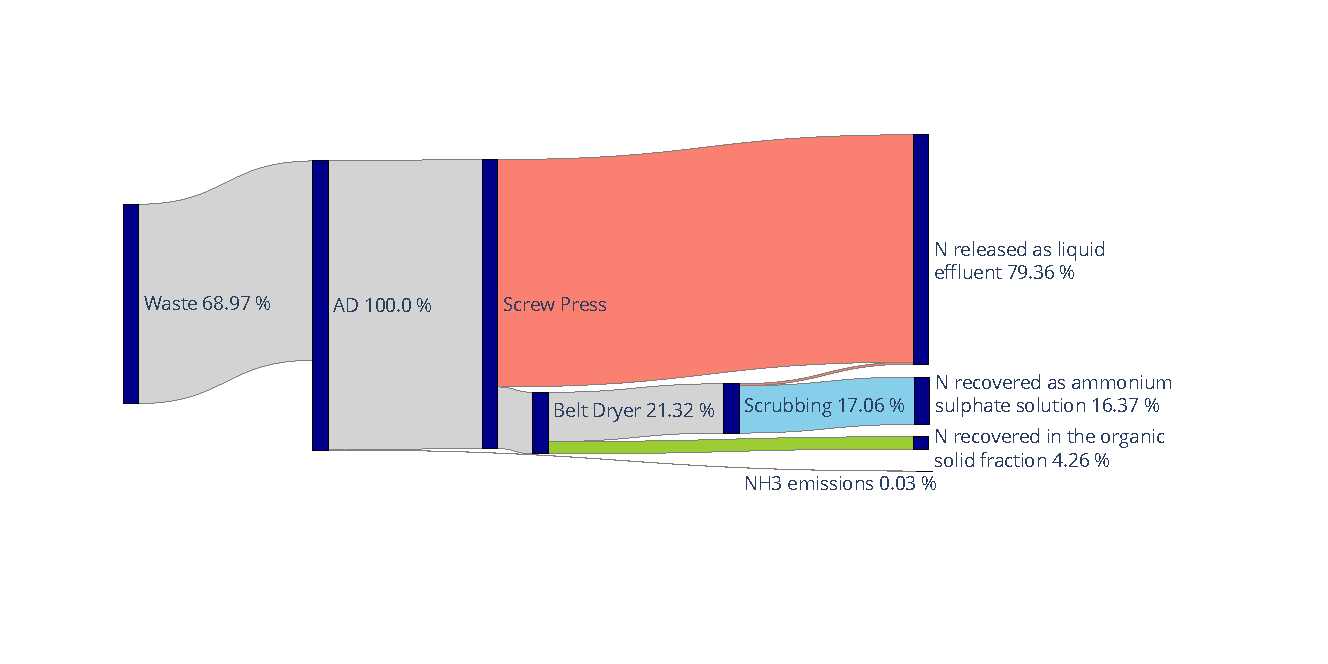
\includegraphics[angle=0, width=0.85\linewidth, trim={2cm 2.8cm 2.5cm 2cm}, clip]{gfx/Chapter6/NitrogenFlow_AmmoniaEvaporation_sankey.pdf}
		\caption{Ammonia evaporation}
		\label{fig:NitrogenFlow_AmmoniaEvaporation_sankey}
	\end{subfigure}
	
	\bigskip
	
	\begin{subfigure}[t]{0.9\textwidth}
		\centering
		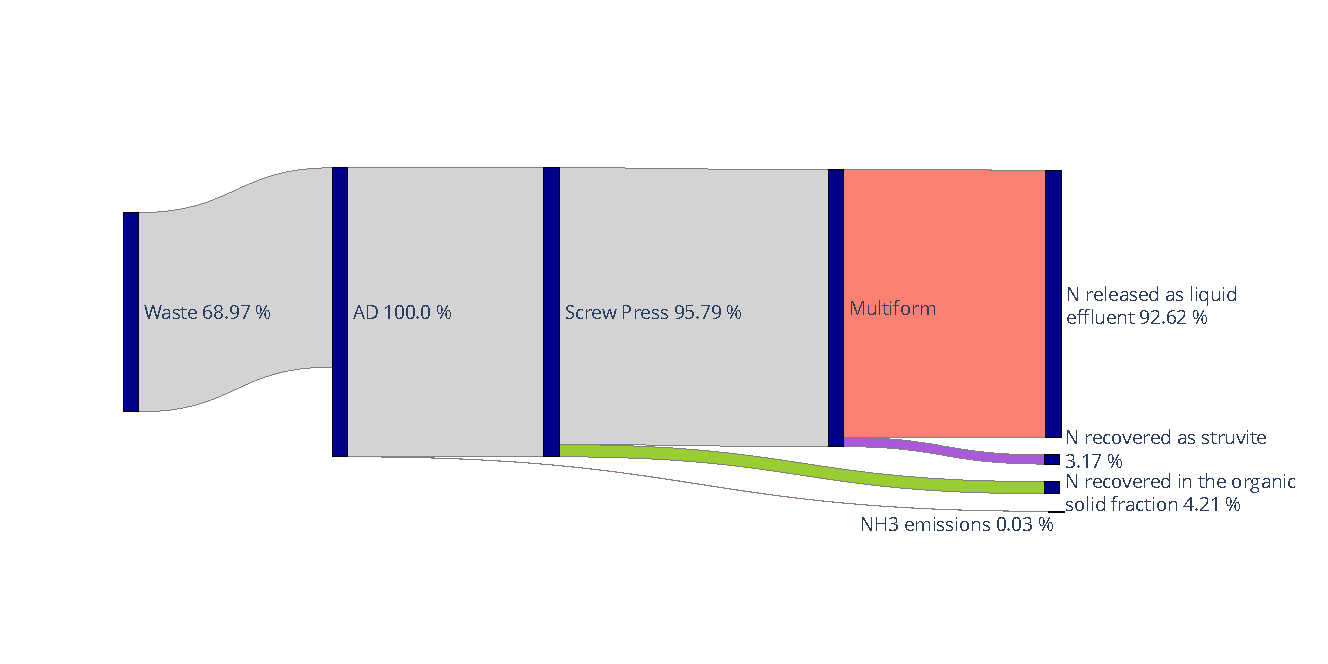
\includegraphics[angle=0,width=\linewidth, trim={2cm 2.5cm 0.5cm 2.5cm}, clip]{gfx/Chapter6/NitrogenFlow_MULTIFORM_sankey.pdf} 
		\caption{Multiform}
		\label{fig:NitrogenFlow_MULTIFORM_sankey}
	\end{subfigure}
	
%	\caption{Relative flows of inorganic nitrogen in the studied processes. Since a fraction of organic nitrogen in swine manure is mineralized after the anaerobic digestion of the waste, the 100\% refers to the inorganic nitrogen in digestate.}
%\end{figure}
%\begin{figure}[h!]	\ContinuedFloat 
%	\centering
	\bigskip
	
	\begin{subfigure}[t]{0.93\textwidth}
		\centering
		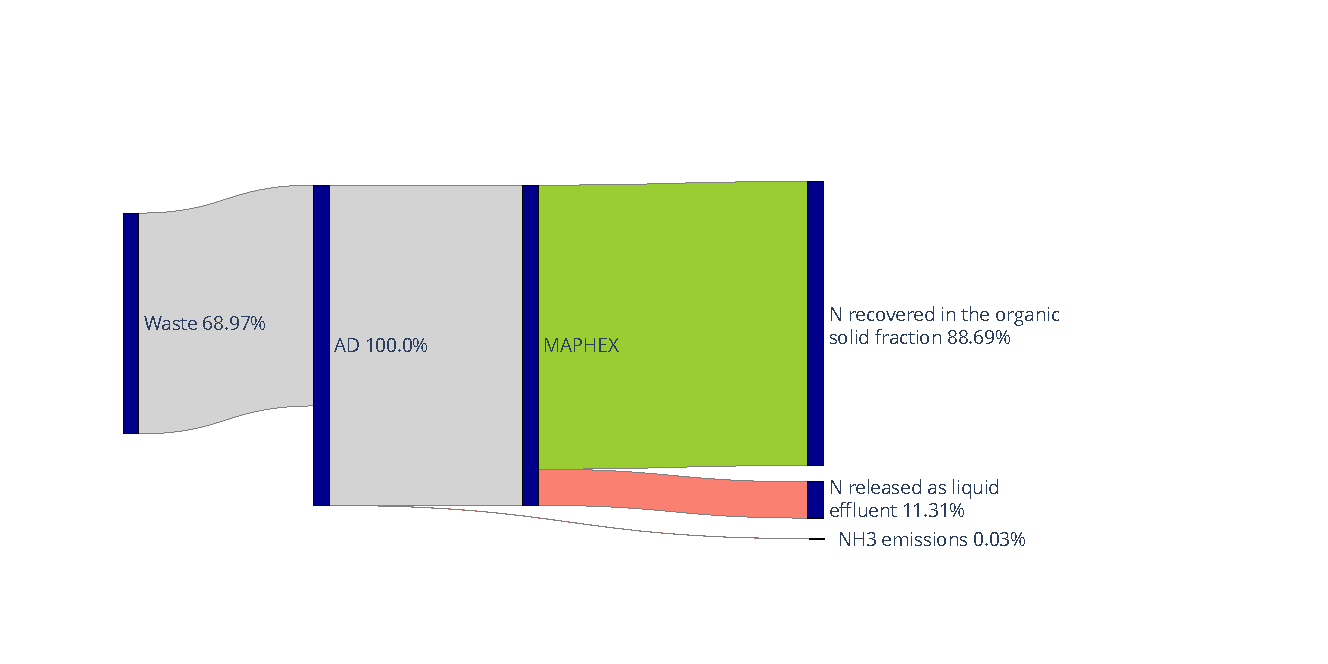
\includegraphics[angle=0,width=0.7\linewidth, trim={1.9cm 2cm 4.5cm 3cm}, clip]{gfx/Chapter6/NitrogenFlow_MAPHEX_sankey.pdf} 
		\caption{MAPHEX}
		\label{fig:NitrogenFlow_MAPHEX_sankey}
	\end{subfigure}
	
	\bigskip
	
	\begin{subfigure}[t]{0.97\textwidth}
		\centering
		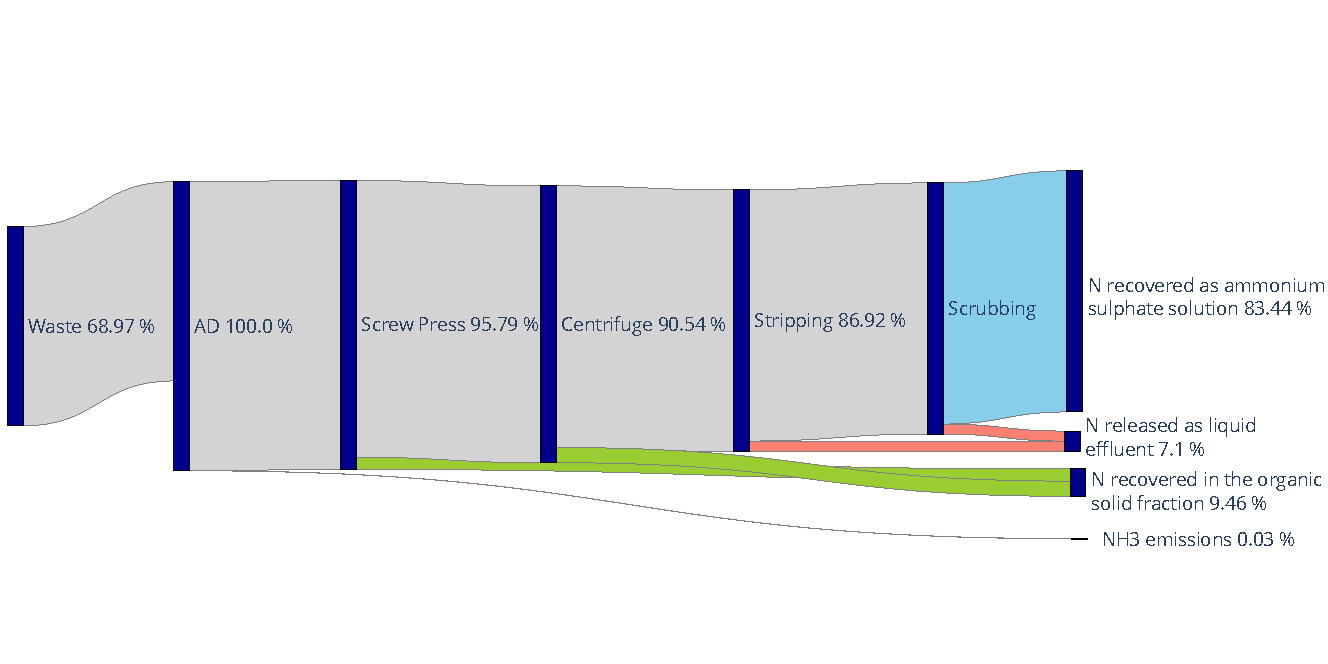
\includegraphics[angle=0,width=\linewidth, trim={0cm 2cm 0cm 3cm}, clip]{gfx/Chapter6/NitrogenFlow_AirStrippingPacked_sankey.pdf} 
		\caption{Stripping in packed tower}
		\label{fig:NitrogenFlow_StrippingPacked_sankey}
	\end{subfigure}

%	\bigskip

	\caption{Relative flows of inorganic nitrogen in the studied processes. Since a fraction of organic nitrogen in swine manure is mineralized after the anaerobic digestion of the waste, the 100\% refers to the inorganic nitrogen in digestate.}

\end{figure}
\begin{figure}[h!]	\ContinuedFloat 
\centering
	
	\begin{subfigure}[t]{0.99\textwidth}
		\centering
		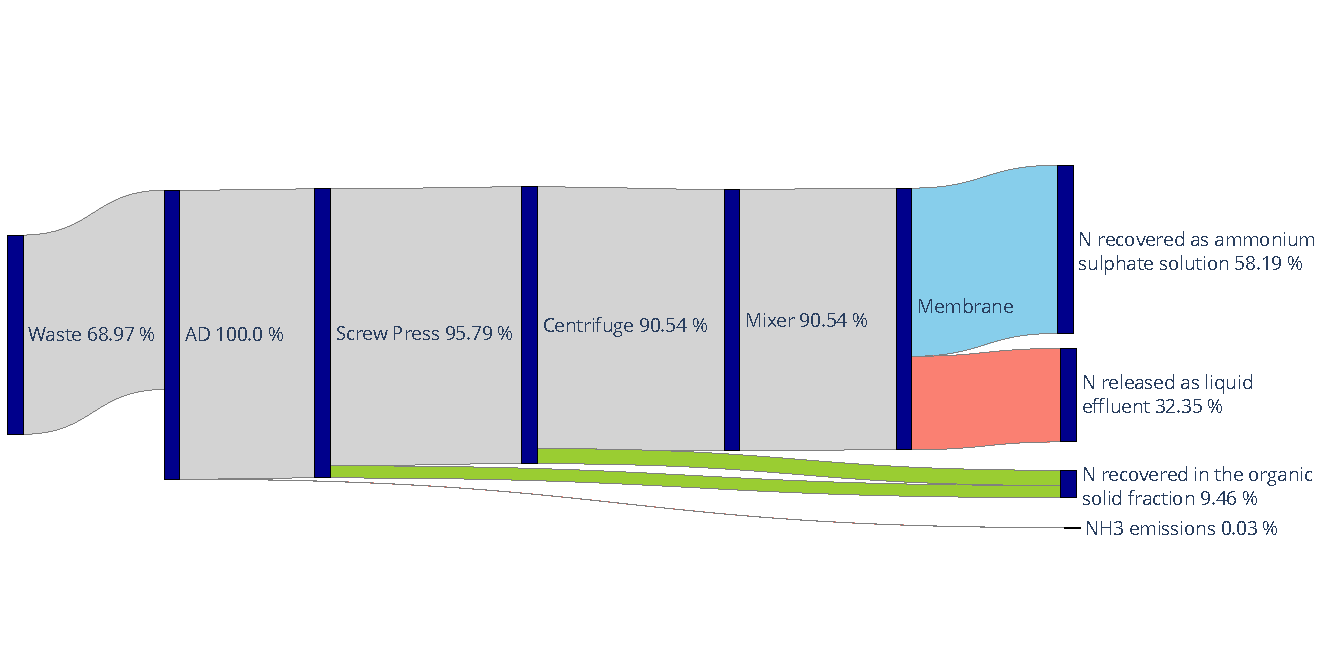
\includegraphics[angle=0,width=\linewidth, trim={0cm 2cm 0cm 2.5cm}, clip]{gfx/Chapter6/NitrogenFlow_Membrane_sankey.pdf} 
		\caption{Membrane}
		\label{fig:NitrogenFlow_Membrane_sankey}
	\end{subfigure}
	
	\caption{Relative flows of inorganic nitrogen in the studied processes. Since a fraction of organic nitrogen in swine manure is mineralized after the anaerobic digestion of the waste, the 100\% refers to the inorganic nitrogen in digestate.}
%	(cont.).
	\label{fig:Sankeys}
\end{figure}

%The efficiency and nitrogen flows for each one of the studied processes are shown in Figure \ref{fig:Sankeys}. Since a fraction of organic nitrogen in swine manure is mineralized after the anaerobic digestion of the waste, the 100\% is referred to the inorganic nitrogen in digestate.
%{\color{red}{
%It can be observed that low nitrogen recovery efficiencies are achieved for digestate drying and struvite production. On the one hand, the recovery of nitrogen through digestate drying is performed through evaporation of the ammonia contained in digestate using a belt dryer. However, this process requires a high solids content of digestate, resulting in low recovery efficiencies due to the discard of a large fraction of the liquid phase of digestate, which contains the most of inorganic nitrogen. On the other hand, the production of struvite from swine waste is limited by the presence of phosphate, which is much lower concentrations that nitrogen, resulting in a low recovery efficiency as well. However, it must be remarked that the product obtained, struvite, is an efective fertilizer with a known composition and easy to be transported, resulting in valuable product \citep{johnston2003effectiveness}. MAPHEX reach a recovery efficiency of up to 88\% though a  serie of physico-chemical separations, resulting in the release of a stream of purified water free of the most fraction of nitrogen. However, in spite of this high efficiency, one of the major drawbacks of this system is the low value of the organic nutrient-rich solid obtained. This solid has a lower density of nutrients than the products obtained by other systems, such as struvite or ammonium sulfate, making the transportation more difficult and expensive, and decreasing its market value.}}

\subsection{Economic assessment and scale-up}

%{\color{red}{OJO Neither uncertaininty}}

%The total cost of nitrogen recovery and waste processing have been estimated for each nitrogen management system evaluated, as shown in Figure \ref{fig:ScaleUGlobal}. These are defined in Eqs. \ref{eq:NRecCost} and \ref{eq:WasteProcCost} respectively for each evaluated technology $i$, where $k$ represents the possible products obtained, $i$ denotes the discount rate (assumed to be 7\%), and $n_{\text{plant}}$ represents the process lifetime, which is assumed to be 20 years. Cost estimation includes OPEX and CAPEX amortization of all equipment involved in the processing of swine waste, as well as incomes from the sales of recovered products sales for those processes producing struvite (Multiform) or ammonium sulphate (digestate drying, stripping in packed tower, and membrane system). CAPEX and OPEX of the systems evalauted are shown in the {\color{blue}{Supplementary Material, Figure 1S}}. The selling prices considered are 0.85 USD per kilogram of struvite \citep{molinos2011economic}, and 0.12 USD per kilogram of ammonium sulphate \citep{AmmoniumSulphatePrice}. The product recovered form MAPHEX system is an solid mainly comprised by organic matter, containing nutrients such as nitrogen and phosphorus. However, since the concentration of nutrients in this material is much lower than struvite or ammonium sulfate, hindering the transportation of this solid, it has been assumed that no incomes can be obtained from this product.

%\begin{align}
%	& Cost_{j}^{\substack{nitrogen\\recovery}} = \frac{OPEX_{j}+CAPEX_{j} \cdot \frac{i \cdot \left( \left(1+i\right)^{n_{\text{plant}}} \right)}{\left( \left( 1+i\right)^{n_{\text{plant}}} -1 \right) } -\sum_{k}{\dot{m}_{j,k} \cdot Price_{k}}}{{\dot{m}_{N_{recovered}}}} \label{eq:NRecCost} \\
%	& Cost_{j}^ {\substack{waste\\processing}} = \frac{OPEX_{j}+CAPEX_{j} \cdot \frac{i \cdot \left( \left(1+i\right)^{n_{\text{plant}}} \right)}{\left( \left( 1+i\right)^{n_{\text{plant}}} -1 \right) } -\sum_{k}{\dot{m}_{j,k} \cdot Price_{k}}}{\dot{m}_{Waste_{processed}}} \label{eq:WasteProcCost}
%\end{align}

The total costs of nitrogen recovery and waste processing for each nitrogen management system evaluated estimated are through Eqs. \ref{eq:NRecCost} and \ref{eq:WasteProcCost}, and shown in Figure \ref{fig:ScaleUGlobal}.
%Figure \ref{fig:ScaleUGlobal} shows the processing cost as a function of the process scale. 
Correlations to estimate the processing cost of the evaluated technologies as a function of animal units are shown in Table \ref{table:ScaleUpCorrelations}. Significant differences on the processing cost of technologies are observed depending on the reference considered for comparison. Considering the cost per kilogram of swine waste, illustrated in Figure \ref{fig:ScaleUp2WasteProcCost}, we observe that Multiform and membrane systems are the processes with the lowest processing cost, 0.13 to 0.02 USD per kg of swine waste processed. 

This approach accounts for operating and amortized capital expenses, as well as for the incomes from the sales of recovered products, as shown in Eq. \ref{eq:WasteProcCost}.
This is a common metric used to measure and compare the processing costs of nitrogen recovery processes \citep{de2019resource, bolzonella2018nutrients}.
However, it does not include the nitrogen recovery efficiency of each process, which can lead to the selection of processes with low waste treatment cost, and low nitrogen recovery efficiency. Therefore, we consider that measuring the processing cost as a function of the recovered nitrogen, as shown in Figure \ref{fig:ScaleUp2}, is a more accurate metric for comparing different systems. Accordingly to this approach, the economic performance of Multiform dramatically decreases as a result of the low nitrogen recovery efficiency of this technology. Conversely, MAPHEX is revealed as more competitive process when the nitrogen recovered is considered. Since MAPHEX is a single size modular technology, its recovery cost shows a linear behavior, slightly affected by adding extra in-parallel modules to process large amounts of waste. Membrane system is the process with the lowest nitrogen recovery cost, from 10.4 to 3.4 USD per kilogram of nitrogen recovered, depending on the waste processing capacity of the system.

We note that the cost of anaerobic digestion stage represents a large fraction of capital expenses. However, this technology might be already implemented in some swine operations. Therefore, the impact of AD in the CAPEX, OPEX and processing costs has been analyzed. Figures \ref{fig:ScaleUGlobal} and {\color{blue}{1S}} show these costs including AD stages, and {\color{blue}{Figures 2S and 3S}} illustrate the costs of nitrogen recovery systems excluding AD. It can be observed that CAPEX costs are significantly higher when AD is considered. This turns into a decrease of processing costs when AD is not considered. Additional correlations for cost estimation
%for this case
are reported in {\color{blue}{Table 1S.}}

%It can be observed in Figure \ref{fig:ScaleUGlobal} that the economies of scale have a large influence in the cost for all the technologies considered. Multiform is the processes that shows the largest cost as a consequence of its low nitrogen recovery efficiency, while digestate drying reveals to be an inexpensive alternative, in spite of the fact that this processes has a relatively low recovery efficient as well. 

\begin{figure}[h]
	\centering 
	\begin{subfigure}[t]{0.455\textwidth}
		\centering
		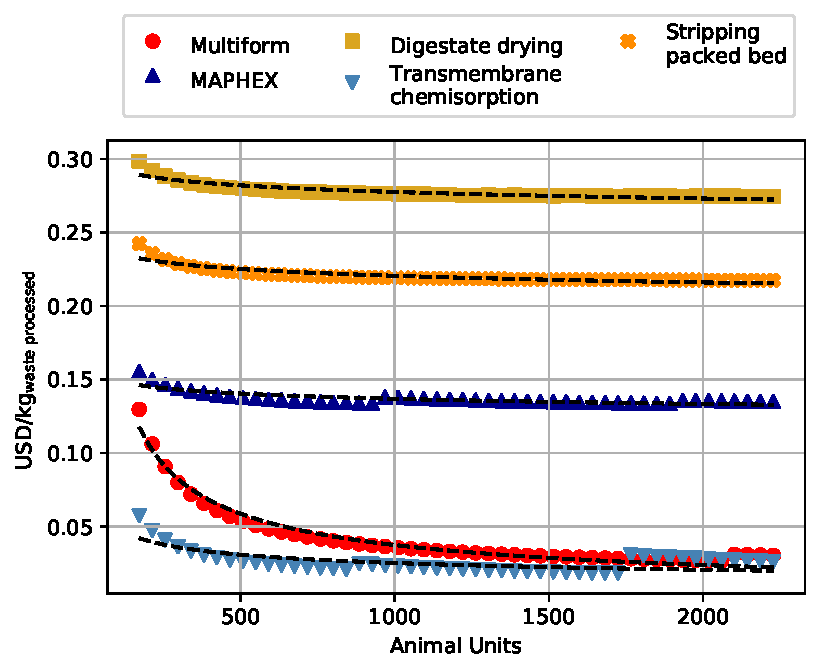
\includegraphics[width=1\linewidth, trim={0cm 0cm 0cm 0cm},clip]{gfx/Chapter6/ScaleUp2WasteProcCost.pdf} 
		\caption{Waste processing cost}
		\label{fig:ScaleUp2WasteProcCost}
	\end{subfigure}
	\begin{subfigure}[t]{0.47\textwidth}
		\centering
		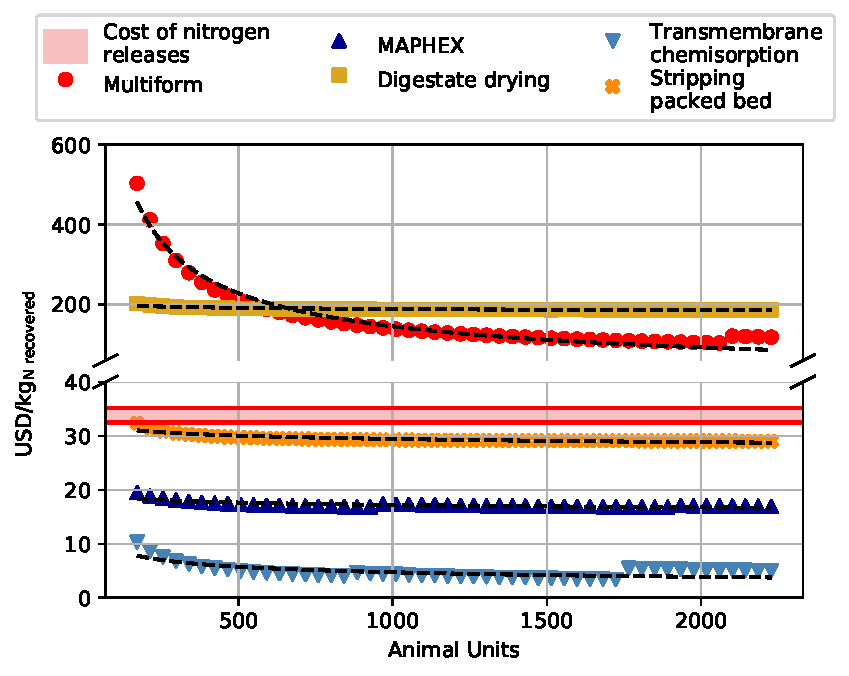
\includegraphics[width=1\linewidth, trim={0cm 0cm 0cm 0cm},clip]{gfx/Chapter6/ScaleUp2.pdf} 
		\caption{Nitrogen recovery cost}
		\label{fig:ScaleUp2}
	\end{subfigure}
	
	\caption{Processing cost for different livestock facility sizes, including the cost of pretreatment and AD stages.} \label{fig:ScaleUGlobal}
\end{figure}

\begin{table}[h] 
	\centering
	\caption{Correlations to estimate the processing cost of the evaluated technologies as a function of animal units ($AU$), including the cost of AD stage.} \label{table:ScaleUpCorrelations}
	\resizebox{\columnwidth}{!}{
	\begin{tabular}{@{}cccc@{}}
		\toprule
		\multirow{2}{*}{System} & &\multicolumn{1}{c}{\begin{tabular}[c]{@{}c@{}}Waste processing cost\\  $\left(\sfrac{\text{USD}}{\text{kg}_{\text{waste processed}}}\right)$\end{tabular}} & \multicolumn{1}{c}{\begin{tabular}[c]{@{}c@{}}Total nitrogen recovery cost\\  $\left(\sfrac{\text{USD}}{\text{kg}_{\text{N recovered}}}\right)$\end{tabular}} \\ \cmidrule(l){3-3}\cmidrule(l){4-4} 
		& Correlation                           & Parameters                &                           Parameters                      \\  \midrule
		%		\cmidrule(l){2-3}
		%		\cmidrule(r){1-1}
		%		Digestate drying 
		Ammonia evaporation 
		& \multirow{13}{*}{$C = a \cdot AU^{b}$}               
		& \begin{tabular}[c]{@{}c@{}}$a$=0.326\\ $b$=-0.0233\end{tabular}  
		& \begin{tabular}[c]{@{}c@{}}$a$=221.805\\ $b$=-0.0233\end{tabular}            \\\\
		Multiform         
		&                                       
		& \begin{tabular}[c]{@{}c@{}}$a$=3.308\\ $b$=-0.648\end{tabular}         
		& \begin{tabular}[c]{@{}c@{}}$a$=12837.477\\ $b$=-0.648\end{tabular}       \\\\
		MAPHEX            
		&                                       
		& \begin{tabular}[c]{@{}c@{}}$a$=0.177 \\ $b$=-0.0372   \end{tabular}       
		& \begin{tabular}[c]{@{}c@{}}$a$=22.240 \\ $b$=-0.0372   \end{tabular}                                             \\ \\ 
		\begin{tabular}[c]{@{}c@{}}Stripping in \\ packed tower  \end{tabular}             &                                       
		& \begin{tabular}[c]{@{}c@{}}$a$=0.271 \\ $b$=-0.0298  \end{tabular}        & \begin{tabular}[c]{@{}c@{}}$a$=36.181 \\ $b$=-0.0298  \end{tabular} \\ \\ 
		Membrane            
		&                                       
		& \begin{tabular}[c]{@{}c@{}}$a$=0.188 \\ $b$=-0.290  \end{tabular}        
		& \begin{tabular}[c]{@{}c@{}}$a$=33.612 \\ $b$=-0.284  \end{tabular}  \\
		\bottomrule 
	\end{tabular}
	}
\end{table}

Additionally, the cost of releasing nitrogen to the environment is illustrated in Figure \ref{fig:ScaleUp2} in order to determine the processes for which nitrogen recovery is more economically beneficial than nitrogen release. The releasing cost of nitrogen is estimated based on the environmental and social cost of atmospheric NH\textsubscript{3} releases, and land, freshwater, and groundwater nitrogen loading. The cost of nitrogen release considering these damages reported by \citet{sobota2015cost} and \citet{compton2017assessing} are 32.5 and 35.15 USD/kg\textsubscript{N released} respectively. We note that the recovery of nitrogen by using membrane systems, MAPHEX, and stripping in packed tower result in economic savings with respect to nitrogen release to the environment. This information can be a driver for the deployment of swine waste treatment processes for nitrogen recovery. However, a debate can be raised regarding what stakeholders should cover the cost of nitrogen recovery from swine industry. 
%The environmental impact from nitrogen releases, and the need of implementing systems for the recovery of nitrogen has been discussed in the introduction section.
%{\color{red}{COMPLETAR ESTO EN LA INTRO}}. 
On the one hand, if nitrogen recovery is not performed at swine facilities, nitrogen releases result in environmental remediation costs in the long-term. These costs are usually covered by national and regional governments, which are ultimately funded by taxpayers. As a result, the environmental impact is covered by all citizens, whether or not they benefit from such businesses. On the other hand, the implementation of nutrient recovery systems could impact the economy of swine farms, which in turn could result in the raise of swine products cost, impacting the final consumers. This approach might seem fairer, since it only involves producers and consumers of swine products. However, it would lead to comparative disadvantages between different swine farms as a result of the savings in nitrogen recovery costs due to the economies of scale, as shown in Figure \ref{fig:ScaleUp2WasteProcCost}. Consequently, small facilities would be more affected by nitrogen recovery than large farms. Therefore, alternative economic schemes should be developed to mitigate the economic impact of the implementation of nitrogen recovery systems at swine facilities. In this regard, previous efforts developed for phosphorus recovery at livestock facilities can be adapted for nitrogen recovery. For instance, the development of a market for trading emissions allowances has been proposed for phosphorus releases from livestock farms \citep{Sampat2}. This scheme can also be explored for nitrogen releases. Additionally, {\color{red}{OJO ACTUALIZAR REFERENCIA!!! \citet{Policies}}} have studied several incentive policies for the implementation of phosphorus recovery systems in livestock facilities, including the fair allocation of limited incentive budgets, which could be adapted to the case of nitrogen recovery.

%{\color{red}{DISCUTIR PRECIOS OBTENIDOS VAN AL REVES QUE EN Nutrients recovery from anaerobic digestate of agro-waste:Techno-economic assessment of full scale applications CUANDPO SE CONSIDERA PRECIO POR KG N RECUPÈRADO EN LUGAR DE JG DE DISGESTATE TRATADO}}

%{\color{red}{INFLUENCE AD IN SUPPLEMENTARY MAT}}

%{\color{red}{CAPEX and OPEX SUPPLEMENTARY MAT}}

%{\color{red}{AU definition}}

%{\color{red}{COMPLETAR ESTO EN LA INTRO}}


%\subsection{Influence of environmental indicators on technology selection}

\section{Conclusions}
%\subsection{Selection of optimal nitrogen management systems}
%\subsection{Assessing the deployment of nitrogen management systems in Castilla y Le\'{o}n}
Intensive swine operations generate  vast amounts of organic waste that it is a source of nitrogen releases into the environment. Since these releases are a significant contributor to the eutrophication of waterbodies, and they can result in harmful environmental impacts such as algal bloom episodes, the recovery of nitrogen at livestock facilities is a desirable measure to reduce the environmental footprint of the food production system.

Several processes have been developed for nitrogen recovery from organic waste, and therefore the selection of the most suitable process has to be addressed considering multiple dimensions, including the nitrogen recovery efficiency, the capital and operating expenses, and the impact of the economies of scale in the final cost of nitrogen recovery. A multi-scale techno-economic study has been performed in order to determine the most suitable nitrogen recovery system based on the waste treatment capacity.
The mass flows throughout all stages from manure collection to the final treatments have been analyzed in order to determine the nitrogen flows throughout each studied system.
%We found that the pretreatment stages, typically liquid-solid separation units, might lead to important losses of nitrogen, and therefore significant losses in nitrogen recovery efficiency. This reduction is specially significant for the recovery of nitrogen by digested drying.
Two metrics have been considered to measure the operating cost of each technology, the waste treatment cost (USD/kg\textsubscript{waste processed}), that it is a metric widely used in literature, and the nitrogen recovery cost (USD/kg\textsubscript{N recovered}). Since the first metric does not account for the nitrogen recovery efficiency of each system, significant differences on the relative performance among the different technologies are found. This is because some technologies that result in low waste treatment costs show low nitrogen recovery efficiencies, resulting in comparatively large nitrogen recovery costs. However, transmembrane chemisorption is revealed as the most cost-effective nitrogen recovery technology, resulting in costs of 0.02-0.06 USD/kg\textsubscript{waste processed}, and 3.4-10.4 USD/kg\textsubscript{N recovered}. Moreover, comparing the negative economic impact of nitrogen releases into the environment, estimated between 32.5 and 35.15 USD/kg\textsubscript{N released} with the cost of nitrogen recovery, three technologies reveal to be economically advantageous, transmembrane chemisorption, MAPHEX, and stripping in packed bed.

Future research is needed to discuss what stakeholders in the production and consumption cycle should assume the costs associated with nitrogen recovery. Additionally, further studies have to be addressed to design and evaluate incentive policies for the effective deployment of nitrogen recovery systems at intensive swine operations.

\section*{Acknowledgments} \label{section:Acknowledgments}
\addcontentsline{toc}{section}{Acknowledgments}
The authors acknowledge funding from the Junta de Castilla y Le\'{o}n, Spain, under grant
%SA026G18 and grant 
EDU/556/2019.

\textbf{Disclaimer:} The views expressed in this article are those of the authors and do not necessarily reflect the views or policies of the U.S. Environmental Protection Agency. Mention of trade names, products, or services does not convey, and should not be interpreted as conveying, official U.S. EPA approval, endorsement, or recommendation. 

\section*{Bibliography}
\addcontentsline{toc}{section}{Bibliography}

\printbibliography[heading=none]
\end{refsection}